% Тут используется класс, установленный на сервере Papeeria. На случай, если
% текст понадобится редактировать где-то в другом месте, рядом лежит файл matmex-diploma-custom.cls
% который в момент своего создания был идентичен классу, установленному на сервере.
% Для того, чтобы им воспользоваться, замените matmex-diploma на matmex-diploma-custom
% Если вы работаете исключительно в Papeeria то мы настоятельно рекомендуем пользоваться
% классом matmex-diploma, поскольку он будет автоматически обновляться по мере внесения корректив
%

% По умолчанию используется шрифт 14 размера. Если нужен 12-й шрифт, уберите опцию [14pt]
%\documentclass[14pt]{matmex-diploma}
\documentclass[14pt]{matmex-diploma-custom}

\usepackage{graphicx}
\usepackage{caption}
\usepackage{subcaption}

\newtheorem{theorem}{Theorem}

\begin{document}
% Год, город, название университета и факультета предопределены,
% но можно и поменять.
% Если англоязычная титульная страница не нужна, то ее можно просто удалить.
\filltitle{ru}{
    chair              = {Кафедра системного программирования},
    title              = {Синтаксический анализ данных, представленных в виде контекстно-свободной грамматики},
    % Здесь указывается тип работы. Возможные значения:
    %   coursework - Курсовая работа
    %   diploma - Диплом специалиста
    %   master - Диплом магистра
    %   bachelor - Диплом бакалавра
    type               = {bachelor},
    position           = {студента},
    group              = 444,
    author             = {Ковалев Дмитрий Александрович},
    supervisorPosition = {к.\,ф.-м.\,н.,\,доц.},
    supervisor         = {Григорьев С.\,В.},
    reviewerPosition   = {программист НИУ ИТМО},
    reviewer           = {Авдюхин Д.\,А.},
    chairHeadPosition  = {д.\,ф.-м.\,н., профессор},
    chairHead          = {Терехов А.\,Н.},
%   university         = {Санкт-Петербургский Государственный Университет},
%   faculty            = {Математико-механический факультет},
%   city               = {Санкт-Петербург},
%   year               = {2013}
}
\filltitle{en}{
    type               = {bachelor},
    chair              = {Chair of Software Engineering},
    title              = {Parsing of the data represented as \\ context free grammar},
    author             = {Dmitry Kovalev},
    supervisorPosition = {associate professor},
    supervisor         = {Semyon Grigorev},
    reviewerPosition   = {Programmer at ITMO University},
    reviewer           = {Avdiukhin Dmitrii},
    chairHeadPosition  = {professor},
    chairHead          = {Christobal Junta},
}

\maketitle
\tableofcontents

\section*{Введение}

Контекстно-свободные грамматики, наряду с регулярными выражениями, активно используются для решения задач, связанных с разработкой формальных языков и синтаксических анализаторов. 
Одним из основных достоинств контекстно-свободных грамматик является возможность задания широкого класса языков при сохранении относительной компактности представления. 
Благодаря данному свойству, грамматики также представляют интерес в такой области информатики, как кодирование и сжатие данных. 
В частности, существует ряд алгоритмов, позволяющих производить сжатие текстовой информации, используя в качестве конечного \cite{sequitur} или промежуточного \cite{Arimura} представления контекстно-свободную грамматику (grammar-based compression). 

Стандартной процедурой при работе с текстовыми данными является поиск в них определенных шаблонов, которые могут быть заданы строкой или регулярным выражением. 
В настоящее время большие объемы информации, как правило, хранятся и передаются по сети в сжатом виде, поэтому актуальной задачей становится поиск шаблонов непосредственно в компактном контекстно-свободном представлении текста.
Такой подход позволяет избежать дополнительных затрат памяти на восстановление исходной формы данных и в некоторых случаях увеличивает скорость выполнения запроса.
Шаблон здесь может быть, как и при поиске в обычном тексте, строкой (compressed pattern matching), сжатой строкой (fully compressed pattern matching) или регулярным выражением.

Известны ситуации, в которых для задания шаблона необходимо использовать более выразительные средства. 
Примером может служить одна из задач биоинформатики --- поиск определенных подпоследовательностей в геноме организма. 
Так, для классификации и исследования образцов, полученных в результате процедуры секвенирования, в них могут искать гены, описывающие специфические рРНК. 
Структура таких генов, как правило, задается при помощи контекстно-свободной грамматики \cite{Anderson2013}. 
Для уменьшения объемов памяти, необходимых для хранения большого количества геномов, используются различные алгоритмы сжатия, в том числе основанные на получении контекстно-свободной структуры исходных последовательностей \cite{galle2011dna}.

Задача поиска КС-шаблонов при использовании КС-представления данных формулируется следующим образом: необходимо найти все строки, принадлежащие пересечению двух языков, один из которых задается грамматикой шаблона, а второй представляет собой язык всех подстрок исходного множества строк, описываемого грамматикой, полученной в результате сжатия данных.
Назовем такой поиск \textit{синтаксическим анализом данных, представленных в виде КС-грамматики}.
%В общем случае задача неразрешима, так как сводится к задаче о проверке пересечения двух языков, порождаемых произвольными КС-грамматиками, на пустоту \cite{harrison1978empt}.
Для постановки экспериментов в области биоинформатики необходимо точнее исследовать возможность проведения синтаксического анализа КС-представления и разработать прототип алгоритма, позволяющего решить данную задачу.
\section{Постановка задачи}
Целью данной работы является разработка алгоритма синтаксического анализа данных, представленных в виде контекстно-свободной грамматики. Для ее достижения были поставлены следующие задачи.
\begin{itemize}
	\item Определить ограничения, при которых синтаксический анализ \linebreak контекстно-свободного представления является разрешимой задачей.
	\item Разработать алгоритм синтаксического анализа КС-представления данных с учетом поставленных ограничений.
	\item Реализовать предложенный алгоритм.
	\item Провести экспериментальное исследование.
\end{itemize}
\chapter{Обзор} \label{relWorks}

В данной главе введены основные термины и определения, используемые в работе, а также рассмотрены основные подходы к анализу встроенных языков и инструменты для их обработки. Также рассмотрен алгоритм обобщённого восходящего синтаксического анализа RNGLR, лежащий в основе разработанного алгоритма. Кроме того, описаны компоненты, использовавшиеся при разработке инструментального пакета YC.SEL.SDK.

\section{Языки и грамматики}

В данном разделе приведён ряд обозначений, понятий и определений из теории формальных языков, которые используются в работе.

\begin{mydef}
    \textbf{Алфавит} $\Sigma$ --- это конечное множество символов.
\end{mydef}

\begin{mydef}
    \textbf{Цепочкой символов} в алфавите $\Sigma$ называется любая конечная последовательность символов этого алфавита. Цепочка, которая не содержит ни одного символа, называется пустой цепочкой. Для её обозначения будем использовать греческую букву $\varepsilon$ (не входит в алфавит $\Sigma$, а только помогает обозначить пустую последовательность символов).
\end{mydef}

\begin{mydef}
    \textbf{Язык} $L$ над алфавитом $\Sigma$ --- это подмножество множества всех цепочек в этом алфавите.
\end{mydef}

\begin{mydef} 
    \textbf{Грамматика} $G$ --- это четвёрка  $\langle T, N, P, S \rangle$, где 
    \begin{itemize}
        \item $T$ --- алфавит терминальных символов или терминалов; 
        \item $N$ --- алфавит нетерминальных символов или нетерминалов, $T \cap N=\varnothing$; 
        \item $P$ --- конечное подмножество множества $(T \cup N)^+ \times (T \cup N)^*$.  Элемент $(a, b) \in P$ называется правилом вывода и записывается в виде $a \rightarrow b$, где $a$ называется левой частью правила, а $b$ --- правой частью, и левая часть любого правила из $P$ обязана содержать хотя бы один нетерминал; 
        \item $S$ --- стартовый символ грамматики, $S  \in N$. 
    \end{itemize}
\end{mydef}

\begin{mydef}    
    \textbf{Вывод цепочки $\omega$ в грамматике $G$.}\\  Цепочка $b \in  ( T \cup  N )^*$ непосредственно выводима из цепочки   $a \in ( T \cup N )^+$ в грамматике $G=\langle T, N, P, S \rangle$  (обозначается  $\rightarrow_G$ ), если  $a = x_1 \cdot y \cdot x_2, b = x_1 \cdot z \cdot x_2$, где $x_1, x_2, y \in   (T \cup N )^*, z \in  (T \cup N )^+$ и правило вывода  $y \rightarrow z$  содержится в $P$. Индекс $G$ в обозначении $\rightarrow_G$ обычно опускают, если $G$ понятна из контекста.

Цепочка $b \in  (T \cup  N )^*$  выводима из цепочки  $a \in (T \cup  N)^+$ в грамматике $G$  (обозначается  $a \Rightarrow_G b$ ), если существуют цепочки $z_0, z_1, \cdots, z_n  (n \geq 0)$, такие, что $a = z_0 \rightarrow z_1 \rightarrow ... \rightarrow z_n = b$ . Последовательность $z_0, z_1, ..., z_n$ называется выводом длины $n$.
\end{mydef}

\begin{mydef}
    \textbf{Язык, порождаемым грамматикой \\ $G = \langle T, N, P, S \rangle$} --- это множество $L(G)  = \{ \omega \in T^* | S \Rightarrow a \}$.
\end{mydef}

\begin{mydef}
    \textbf{Левосторонний вывод цепочки $\omega$ в грамматике  $G~=~\langle T,~N,~P,~S \rangle$}~--- это вывод, в котором на каждом шаге заменяется самое левое из всех вхождений нетерминальных символов, то есть каждый шаг вывода имеет вид $u A \theta \Rightarrow u \beta \theta$, где $( A \rightarrow \beta ) \in P$, $u \in \Sigma ^*$ и $\theta \in (N \cup \Sigma)^* $.
\end{mydef}

\begin{mydef}    
    \textbf{Правосторонний вывод цепочки $\omega$ в грамматике $G=\langle  T, N, P, S  \rangle$} определяется аналогично левостороннему, то есть на каждом шаге заменяется самое правое вхождение нетерминала.
\end{mydef}

\begin{mydef}    
    Грамматика $G$ называется \textbf{неоднозначной} (ambiguous), если существует слово $\omega \in L(G)$, которое имеет два или более левосторонних вывода. В противном случае контекстно-свободная грамматика называется \textbf{однозначной} (unambiguous). 
\end{mydef}

\begin{mydef}    
    Язык $L_1$ называется \textbf{существенно неоднозначным}, если не существует такой грамматики $G$, что $G$ однозначна и $L_1 = L(G)$. 
\end{mydef}

\begin{mydef}
    \textbf{Деревом вывода} цепочки $\omega \in T^*$ в грамматике $G=\langle T, N, P, S \rangle$ называется упорядоченное дерево со следующими свойствами. 
\begin{itemize}
    \item Корень помечен $S$.

    \item Если его внутренний узел помечен $A \in N$ и $X_1, \ldots , X_k \in T \cup N$ ---   перечисленные слева направо пометки всех сыновей этого узла, то правило $A \rightarrow X_1 \ldots X_k \in P$.

    \item Если его внутренний узел помечен $A \in N$ и $\varepsilon$ --- пометка единственного сына этого внутреннего узла, то правило $A \rightarrow \varepsilon \in P$.

    \item $\omega = a_1 \ldots a_m$, где $a_1, \ldots , a_m \in T \cup \{\varepsilon\} $ перечисленные слева направо пометки всех листьев этого дерева.
    
\end{itemize}
\end{mydef}

\begin{mydef}    
    \textbf{Динамически формируемое строковое выражение} --- это строковое выражение, значение которого будет известно только в момент выполнения программы.
    \end{mydef}
    \begin{mydef}    
     Язык, на котором написана программа, будем называть \textbf{внешним языком}.
     \end{mydef}
     
      В случае, когда известно, что значение строкового выражения должно являться кодом на некотором языке, говорят о \textbf{встроенных языках} (также называемых встроенными строковыми языками или string-embedded languages~\cite{Alvor1}). Например, для листинга~\ref{lst:stringExpr} внешним языком является C\#. Про переменную \verb|sExec|, основываясь на строках 3--7, можно сделать предположение, что она должна содержать выражение на SQL. Таким образом, в данном примере присутствует SQL, встроенный в C\#, и динамически формируемый SQL-запрос. Отметим, что выражение на строке 9 является статическим, а строковое выражение на строке 10 является динамически формируемым, но не является кодом на некотором языке программирования. Обработка таких выражений в общем случае называется анализом строк (string analysis~\cite{StringAnalysis}).


\fvset{frame=lines,framesep=5pt}
\begin{listing}
    \begin{pyglist}[language=csharp,numbers=left,numbersep=5pt]

public void Example(string tbl, bool cond)
{
    string sExec =
        "SELECT sOrderDescription, cderitInfo, @sMagicKey FROM ts."
        + tbl;
        + (cond ? "WHERE fld = 1 " : "WHERE fld = 2 ");

    db.Execute(sExec);
    
    Console.WriteLine("Success. Table: " + tbl);
}
\end{pyglist}
\caption{Пример кода метода на языке программирования C\#, содержащего динамически формируемые строковые выражения}
\label{lst:stringExpr}
\end{listing}

Одним из распространённых способов классификации грамматик является иерархия грамматик по Хомскому~\cite{chomsky}. Рассмотрим её более подробно, так как различия между классами играют важную роль в решении задач данной работы.

\begin{itemize}
    \item \textbf{Грамматика типа 0.} Любая грамматика является грамматикой типа 0. На вид правил грамматик этого типа не накладывается никаких дополнительных ограничений. Класс языков типа 0 совпадает с классом рекурсивно перечислимых языков.
    
    \item \textbf{Грамматикой типа 1} будем называть неукорачивающую грамматику. Грамматика $G = \langle T, N, P, S \rangle$ называется неукорачивающей, если правая часть каждого правила из $P$ не короче левой части: для любого правила $\alpha \rightarrow \beta \in P$ выполняется неравенство $| \alpha | <= | \beta |$. В виде исключения в неукорачивающей грамматике допускается наличие правила $S \rightarrow \varepsilon$, при условии, что $S$ не встречается в правых частях правил. Тип 1 также можно определить с помощью контекстно-зависимых грамматик. Грамматика $G = \langle T, N, P, S \rangle$ называется контекстно-зависимой (КЗ), если каждое правило из $P$ имеет вид $\alpha \rightarrow \beta$, где $\alpha = \omega_1 A\omega_2, \beta = \omega_1\gamma\omega_2, A \in N, \gamma \in (T \cup N )^+   , \omega_1, \omega_2 \in (T \cup N)^*$. В виде исключения в КЗ-грамматике допускается наличие правила с пустой правой частью $S \rightarrow \varepsilon$, при условии, что $S$ не встречается в правых частях правил. Цепочку $\omega_1$ называют левым контекстом, цепочку $\omega_2$ называют правым контекстом. Язык, порождаемый контекстно-зависимой грамматикой, называется контекстно-зависимым языком. 
    
    \item \textbf{Грамматикой типа 2} будем называть контекстно-свободную грамматику. Грамматика $G = \langle T, N, P, S \rangle$ называется контекстно-свободной (КС), если каждое правило из $P$ имеет вид $A \rightarrow \beta, где A \in N, \beta \in ( T \cup N )^*$. Заметим, что в КС-грамматиках допускаются правила с пустыми правыми частями.  Язык, порождаемый контекстно-свободной грамматикой, называется контекстно-свободным языком. 

    \item \textbf{Грамматикой типа 3} является регулярня грамматика, определение которой приведено ниже.
     
\end{itemize}

Грамматика $G = \langle T, N, P, S \rangle$ называется праволинейной, если каждое правило из $P$ имеет вид $A \rightarrow wB$ либо $A \rightarrow w$, где $A, B \in N, w \in T*$. Грамматика $G = \langle T, N, P, S \rangle$ называется леволинейной, если каждое правило из $P$ имеет вид $A \rightarrow Bw$ либо $A \rightarrow w$, где $A, B \in N, w \in T*$. 

При фиксированном языке $L$ два следующих утверждения эквивалентны: 
\begin{itemize}
    \item существует праволинейная грамматика $G_1$, такая что $L = L(G_1)$; 
    \item существует леволинейная грамматика $G_2$, такая что $L = L(G_2)$.
\end{itemize}

Из данного утверждения следует, что праволинейные и леволинейные грамматики определяют один и тот же класс языков, который будем называть классом регулярных языков. Право- и леволинейные грамматики будем называть \textbf{регулярными грамматиками}. 

    Существуют различные способы описания языков. Если язык конечен, то его можно описать  простым перечислением входящих в него цепочек. Однако формальный язык может быть бесконечным, и в таком случае требуются механизмы, позволяющие конечным образом представлять бесконечное множество цепочек. Можно выделить два основных подхода для такого представления:
\begin{enumerate}
    \item механизм распознавания, когда описывается процедура, проверяющая принадлежность цепочки описываемому языку;
    \item механизм порождения (генерации), когда задаётся механизм, способный построить все цепочки описываемого языка.
\end{enumerate}

     Основной способ реализации механизма порождения --- использование грамматик, которые как раз и описывают правила построения цепочек некоторого языка. Вместе с этим, можно явным образом описать процедуру-генератор цепочек языка, что также будет являться описанием языка. Например, программа на любом языке программирования, генерирующая некоторый текст, является описанием языка. В данной работе будут рассматриваться такие программы.


\section{Конечные автоматы и преобразователи}

Одним из способов задания регулярных языков является описание конечного автомата, который может быть использован и как генератор, и как распознаватель.

\begin{mydef}
\textbf{Конечный автомат} (Finite State Automata,~\cite{FSA}) --- это пятёрка $M = \langle Q,\Sigma,\Delta,I,F \rangle$, где:
\begin{itemize}
    \item $\Sigma$ --- конечный алфавит;
    \item $Q$ --- конечное множество состояний;
    \item $I$ --- множество начальных состояний, $I \subseteq Q$;
    \item $F$ --- множество заключительных или допускающих состояний, $F \subseteq Q$;
    \item $\Delta \subseteq Q \times \Sigma ^ * \times Q$; если $\langle p, x, q \rangle \in \Delta$, то $\langle p, x, q \rangle$ называется переходом (transition) из $p$ в $q$, а слово $x$ --- меткой (label) этого перехода; в общем случае автомат является недетерминированным (НКА), то есть позволяющим несколько переходов с одинаковым начальным состоянием и одинаковой меткой.
\end{itemize}
\end{mydef}

\begin{mydef}
Конечный автомат $\langle Q , \Sigma , \Delta , I , F \rangle$ называется \textbf{детерминированным} (deterministic) (ДКА), если 
\begin{itemize}
    \item множество $I$ содержит ровно один элемент;
    \item для каждого перехода $\langle p , x , q \rangle \in \Delta$ выполняется равенство $|x| = 1$;
    \item для любого символа $a \in \Sigma$ и для любого состояния $p \in Q$ существует не более одного состояния $q \in Q$ со свойством $\langle p , a , q \rangle \in \Delta$.
\end{itemize}
\end{mydef}

\begin{mydef}
Конечный автомат с $\varepsilon$-переходами --- это конечный автомат, в котором есть возможность совершать переходы по $\varepsilon$.
\end{mydef}

\begin{mydef}
\textbf{$\varepsilon$-НКА $A$} --- это НКА, где  $\delta : Q\times (\Sigma\cup\{\varepsilon\}) \to 2^Q$.
\end{mydef}

\begin{mydef}
 \textbf{Язык, распознаваемый конечным автоматом $M$,} --- это язык $L(M)$, состоящий из всех допускаемых данным автоматом цепочек. Также говорят, что автомат $M$ описывает или задаёт некоторый язык $L(M)$.
\end{mydef}

Класс регулярных языков эквивалентен классу конечных автоматов в том смысле, что для любого регулярного языка $L_1$ можно построить детерминированный конечный автомат $M$, такой $ L(M)=L_1 $. При этом множество языков, допускаемых автоматами с $\varepsilon$-переходами, совпадает с множеством языков, допускаемых детерминированными конечными автоматами. Также будет удобно отождествлять регулярный язык и регулярное множество.

Конечные автоматы можно изображать в виде диаграмм переходов (transition diagram). На диаграмме каждому состоянию соответствует вершина графа, а переходу --- дуга. Дуга из $p$ в $q$, помеченная словом $x$, означает, что $\langle p , x , q \rangle$ является переходом данного конечного автомата. Вершины, соответствующие начальным и конечным состояниям, отмечаются отдельно: конечные состояния изображаются как двойной круг, начальные отмечаются отдельной входной дугой, не имеющей стартовой вершины. Также в данной работе будет использоваться следующая цветовая нотация: конечные вершины обозначены красным цветом, начальные --- зелёным.  Таким образом, автомат представим в виде графа и в данной работе к конечным автоматам будет применяться терминология из теории графов.

В рамках рассматриваемой предметной области конечные автоматы широко применяются для приближения множества возможных значений динамически генерируемой программы~\cite{Alvor1, JSA, RegOverApprox}: в результате анализа программы-генератора строится конечный автомат, описывающий регулярное множество $R$, являющееся приближением множества генерируемых программ $S$. При решении многих задач необходимо, чтобы $R$ было приближением $S$ сверху, то есть выполнялось включение $R \supseteq S$. Например, при поиске ошибок это позволит оценивать полноту анализа: если алгоритм не выявил некорректных цепочек в $R$, то их точно нет и в $S$. Однако возможны ложные срабатывания: алгоритм обнаружил некорректную цепочку $\omega \in R$, но $\omega \not\in S, \omega \in R-S$. Для того, чтобы минимизировать количество промахов, необходимо уменьшать $R-S$, то есть строить как можно более точное приближение. В работе~\cite{RegOverApprox} предлагается алгоритм построения такого приближения. Он будет использоваться в данной работе.

\begin{mydef}

\textbf{Конечный преобразователь} (Finite State Transducer,~\cite{FST}) {---} это конечный автомат, который может возвращать конечное число символов для каждого входного символа. Конечный преобразователь может быть задан следующей шестёркой элементов: $\langle Q, \Sigma, \Delta, q_0, F, E \rangle$, где:

\begin{itemize}
\item $Q$ --- множество состояний; 
\item $\Sigma$ --- входной алфавит;
\item $\Delta$ --- выходной алфавит; 
\item $q_0 \in Q$ --- начальное состояние;
\item $F \subseteq Q$ --- набор конечных состояний; 
\item $E \subseteq Q \times (\Sigma \cup \{\varepsilon\}) \times (\Delta \cup \{\varepsilon\})  \times Q$ --- набор переходов. 
\end{itemize}

\end{mydef}

Конечные преобразователи находят широкое применение в области обработки естественного языка (Natural Language Processing \cite{Mohri}). Кроме этого, они используются и при проведении лексического анализа, который является переводом входной цепочки из одного языка в другой: из языка над алфавитом символов в язык над алфавитом терминалов. Большинство генераторов лексических анализаторов строят по описанию лексики языка соответствующий конечный преобразователь.

Важной операцией над конечными преобразователями является операция композиции. \textbf{Композиция} конечных преобразователей~{---}~это два последовательно  взаимодействующих конечных преобразователя, работающих следующим образом: выход первого конечного преобразователя подаётся на вход второму, что позволяет описывать цепочки трансформаций. Ниже дано формальное определение операции композиция над конечными преобразователями, допускающие наличие $\varepsilon$-переходов.

\begin{mydef}

\textbf{Композицией} двух конечных преобразователей \\  $T_1~=~\langle Q_1, \Sigma_1, \Delta_1, q_{0_{1}}, F_1, E_1 \rangle$ и $T_2~=~\langle Q_2, \Sigma_2, \Delta_2, q_{0_{2}}, F_2, E_2 \rangle$ является конечный преобразователь  $T =\langle Q_1  \times Q_2, \Sigma_1, \Delta_2, \\ \langle q_{0_{1}}, q_{0_{2}} \rangle, F_1 \times F_2, E \cup E_{\varepsilon} \cup E_{i,\varepsilon} \cup E_{o,\varepsilon} \rangle$, где: 

\begin{itemize}
\item $E = \{ \langle \langle p, q \rangle, a, b, \langle p', q' \rangle \rangle\ | \exists c \in \Delta_1 \cap \Sigma_2 : \langle p, a, c, p' \rangle \in E_1 \wedge \langle q, c, b, q' \rangle \in E_2\}$;
\item $E_{\varepsilon} = \{ \langle \langle p, q \rangle, a, b, \langle p', q' \rangle \rangle\ | \langle p, a, {\varepsilon}, p' \rangle \in E_1 \wedge \langle q, {\varepsilon}, b, q' \rangle \in E_2\}$;
\item $E_{i, \varepsilon} = \{ \langle \langle p, q \rangle, {\varepsilon}, a, \langle p, q' \rangle \rangle\ | \langle q, {\varepsilon}, a, q' \rangle \in E_2 \wedge p \in Q_1 \} $;
\item $E_{o, \varepsilon} = \{ \langle \langle p, q \rangle,  a, {\varepsilon}, \langle p', q \rangle \rangle\ | \langle p, a, {\varepsilon}, p' \rangle \in E_1 \wedge q \in Q_2 \}. $
\end{itemize}
\end{mydef}

В рамках данной работы конечные преобразователи и их композиция будут использоваться для лексического анализа динамически формируемых строковых выражений.

\section{О применимости статического анализа строковых выражений}

Статический анализ динамически формируемых выражений полезен на различных этапах работы с кодом при решении различных задач~\cite{DevelopmentDSQLTools}. Рассмотрим пример и поясним, какие задачи необходимо решать и каким образом анализ строковых выражений помогает решать данные задачи. Мы рассмотрим пример встроенного SQL, однако все рассмотренные задачи актуальны и для других языков.

\fvset{frame=lines,framesep=5pt}
\begin{listing}
    \begin{pyglist}[language=csharp,numbers=left,numbersep=5pt]

public void NewReport(int prodId = 0, int status = 0, int nType = 0)
{
    int nProdIdL = prodId;

    string sMagicKey = "[" + prodId.ToString() + "]";

    string tbl = status == 0 ? "InOrders " : "OutOrders ";

    while (nProdIdL > 0)
    {
        sMagicKey = "[" + sMagicKey + "]";
        nProdIdL = nProdIdL - 1;
    }

    string sExec =
        "SELECT sOrderDescription, cderitInfo, " + sMagicKey
        + " FROM ts." + tbl +
        "as t1 JOIN tCreData cd (NOLOCK) ON cd.ncredataid "
        + " = t1.ncredataid";

    string sWhere = nType == 0
        ? "WHERE nOrderType = 0 AND nStatus > 2 "
        : "WHERE nStatus > 0 ";

    sExec = "INSERT INTO reports (description, creditInfo, id)"
            + " VALUES " + sExec + sWhere;

    db.Execute(sExec);
}
\end{pyglist}
\caption{Пример кода метода на языке программирования C\#, формирующего и выполняющего динамический SQL-запрос}
\label{lst:csqlExample}
\end{listing}

Одной из широко распространённых задач, является оценка качества кода и его сложности с использованием различных формальных метрик~\cite{SoftwareMetrics}. При вычислении таких метрик важно учитывать, что использование динамически формируемых выражений, сложность их конструирования, количество и содержание возможных значений и многие другие характеристики сказываются на качестве и сложности содержащего их кода. По этой причине необходимо иметь возможность оценивать сложность динамически формируемых выражений с различных точек зрения~\cite{DSQLQualityMesure,DSQLQualityMesureBIG}. С одной стороны, необходимо оценивать сложность формирования выражения. Так в примере, представленном в листинге~\ref{lst:csqlExample}, для формирования запроса используется цикл (строки 9--13), что может приводить к потенциально бесконечному множеству различных значений выражения и усложнять процесс сопровождения. С другой стороны, важна сложность возможных значений выражения. В листинге~\ref{lst:csqlExample}, в динамически формируемом запросе используется конструкция соединения таблиц (\verb|JOIN|, строка 17). Большое количество соединений и сложность условий часто становится причиной проблем с производительностью и может служить признаком неудачного дизайна схемы данных~\cite{DSQLQualityMesureBIG}.

Другой набор задач, связанный с сопровождением и модификацией систем, разработанных с активным использованием динамически формируемых выражений --- это  извлечение знаний о системе~\cite{DSQLSemaFRecovery} и автоматизированный реинжиниринг программного обеспечения~\cite{DSQLReverseEngineering}. Например, при активном использовании встроенного SQL может возникать задача анализа или восстановления схемы данных~\cite{DevelopmentDSQLTools}. Проанализировав структурное представление динамически формируемого SQL-кода в примере из листинга~\ref{lst:csqlExample}, можно сделать вывод о том, что данный код обращается к таблицам \verb|InOrders|, \verb|OutOrders| и \verb|tCreData| на чтение, а к таблице \verb|reports| на запись. Без анализа строковых выражений эта информация не может быть получена, а она может быть полезна, например, при модификации схемы данных.

Так как встроенные языки активно используются на практике, то важна их поддержка в интегрированных средах разработки, что может быть полезно не только при непосредственной разработке, но и при автоматизированном и ручном изучении кода, совмещённом с решением перечисленных выше задач. Дополнительная поддержка встроенных языков в средах разработки может включать подсветку синтаксиса и парных элементов, навигацию по коду с учётом динамически формируемого выражения, диагностику и подсветку ошибок, что упрощает работу с кодом. Например, в листинге~\ref{lst:csqlExample} пропущен пробел между блоком \verb|WHERE| (переменная \verb|sWhere|, строки 20--22) и началом конструкции \verb|SELECT| (переменная \verb|sExec|, строки 15--18). То есть при выполнении данного метода будет формироваться некорректный запрос, но об этом станет известно только в момент выполнения метода. Однако ошибки такого рода можно обнаруживать без запуска программы и сообщать об этом разработчику.

\section{Подходы к анализу встроенных языков}\label{SELAnalysisDescr}

Анализ динамически формируемых выражений актуален как в задачах обеспечения безопасности программного обеспечения (поиск мест в коде, уязвимых для SQL-инъекций~\cite{SQLInjection}), так и для разработки, сопровождения и модернизации систем, разработанных с применением встроенных языков. Для решения подобных задач существует ряд различных подходов, основные из которых рассмотрены ниже.

Существуют два класса подходов к анализу программного кода: динамический и статический. Статический анализ подразумевает !!!!Динамический анализ ~\cite{DynamicDSQLTranslation} ...  Плюсы, минусы.

\textbf{Проверка включения языков.} В рамках данного подхода в результате анализа внешнего кода строится язык $L_1$, являющийся приближением языка $L$, генерируемого программой. После чего проверяется включение $L_1$ в язык $L_2(G)$, описанный эталонной грамматикой $G$. Основной недостаток данного подхода --- невозможность получить какую-либо информацию, кроме знания о вхождении или не вхождении одного языка в другой. Как следствие, проведение более сложных видов статического анализа или трансформации невозможно. Можно выделить несколько вариантов данного подхода, различающихся классом языка $L_1$.

\begin{itemize}
    \item Регулярная аппроксимация: $L_1$ является регулярным языком. Однако язык $L$ не обязан быть регулярным, так как программа-генератор может быть реализована на тьюринг-полном языке, что может приводить к существенной потере точности при построении приближения. Достоинством такого подхода является разрешимость задачи проверки включения $L_1$ в $L_2$ для регулярных $L_1$ и $L_2$, являющегося однозначным контекстно-свободным языком~\cite{LangIncusion}. Инструмент, реализующий данный подход, --- Java String Analizer~\cite{JSA}, являющийся анализатором строковых выражений в коде на Java.

    \item Контекстно-свободное приближение: $L_1$ является контекстно-свободным языком.  Достоинством такого приближения является его б\'{о}льшая точность, однако проверка включения одного контекстно-свободного языка в другой является неразрешимой в общем случае задачей~\cite{LangIncusion}. По  этой причине при использовании такого приближения будет получено неточное решение, так как потребуется применение эвристик. Данный подход реализован в инструменте PHPSA~\cite{PHPSA}, предназначенном для проверки корректности динамически формируемых программами на PHP выражений.

\end{itemize}

\textbf{Синтаксический анализ.} Данный подход основан на применении техник синтаксического анализа для работы с динамически формируемыми выражениями. Благодаря этому, кроме проверки корректности выражений, становится возможным решение более сложных задач, требующих знаний о структуре вывода или работы с деревом разбора, таких как семантический анализ или трансформации. Ниже перечислены существующие на текущий момент варианты данного подхода.

\begin{itemize}
    \item Абстрактный LR-анализ. В исследованиях группы во главе  с Kyung-Goo Doh (Hanyang University, South Korea) предлагается комбинация анализа потока данных и синтаксического анализа на основе LALR(k) алгоритма, позволяющая строить множество LR-стеков для всех значений строкового выражения~\cite{LrAbstract1, LrAbstract2, LRAbstractParsingSema}. Так как задача проверки включения для двух контекстно-свободных языков неразрешима, то представлено приближённое решение. В работе~\cite{LRAbstractParsingSema} обоснована возможность семантического анализа на основе классического для LR-анализа механизма: атрибутных грамматик~\cite{Dragon} и выполнения семантического действия при выполнении свёртки. Однако не до конца исследована эффективность данного подхода при работе с семантическими действиями, требующими больших ресурсов при вычислении.

    \item Синтаксический анализ регулярного множества. Для языка $L$ строится регулярная аппроксимация. Далее над построенной аппроксимацией решаются задачи лексического и синтаксического анализа. Данный подход рассмотрен в работах~\cite{Alvor1, Alvor2} и реализован в инструменте Alvor. Данный инструмент является плагином к среде разработки Eclipse, предоставляющим поддержку встроенного SQL в Java: статический поиск ошибок, тестирование запросов в базе данных. Достоинством такого подхода является разделение обработки на независимые шаги: построение аппроксимации, лексический анализ, синтаксический анализ~\cite{Alvor2}. Это позволяет более гибко переиспользовать существующие реализации тех или иных шагов и упрощает создание нового инструмента на базе имеющихся. Использование атрибутных грамматик --- классического для LR-анализа способа задания семантики --- и построение леса разбора в рамках данного подхода также не обсуждается.

\end{itemize}


\section{Обзор инструментов для работы со встроенными языками}\label{SELToolsDescr}

    Задачи анализа динамически формируемых строковых выражений возникают в различных контекстах и применительно к различным языкам, что приводит к появлению разнообразных программных инструментов.

    Среди языков, код на которых динамически формируется в виде строк, одним из наиболее распространённых является SQL с его многочисленными диалектами.  При этом часто используется динамический SQL: генерация выражений на SQL в рамках кода на SQL, часто в хранимых процедурах. Одна из актуальных задач, при решении которой необходимо обрабатывать динамический SQL, --- это миграция приложений баз данных. Для её решения существует ряд промышленных инструментов. В силу особенностей решаемой задачи нас интересуют инструменты для трансляции хранимого кода приложений баз данных. Самыми известными в данной области являются такие инструменты как PL-SQL Developer~\cite{PLSQLDeveloper}, SwisSQL~\cite{SwissSQL}, SQL Ways~\cite{SQLWays}. Эти инструменты применяются для трансляции хранимого SQL-кода, однако только SQL Ways обладает возможностью трансформации строковых SQL-запросов в ряде простых случаев. Динамически формируемые запросы со сложной логикой построения не поддерживаются современными промышленными инструментами.
    
    Далее рассмотрим инструменты, которые изначально ориентированы на решение различных задач анализа динамически формируемых выражений. Многие из них предназначены для предоставления поддержки встроенных языков в интегрированных средах разработки. Как правило, эти инструменты реализуют один из основных подходов, описанных в разделе~\ref{SELAnalysisDescr}.

\textbf{Java String Analyzer} (JSA, \cite{JSA, JSAUrl}) {---}  инструмент для анализа строк и строковых операций в программах на Java. Основан на проверке включения регулярной аппроксимации встроенного языка в контекстно-свободное описание эталонного. Для каждого строкового выражения строится конечный автомат, представляющий приближенное значение всех значений этого выражения, которые могут быть получены во время выполнения программы. Для того, чтобы получить этот конечный автомат, необходимо из графа потока данных анализируемой программы построить контекстно-свободную грамматику, которая получается в результате замены каждой строковой переменной нетерминалом, а каждой строковой операции {---} правилом продукции. После этого полученная грамматика аппроксимируется регулярным языком. В качестве результата работы данный инструмент также возвращает строки, которые не входят в описанный пользователем язык, но могут сформироваться во время исполнения программы. 

\textbf{PHP String Analyzer} (PHPSA, \cite{PHPSA, PHPSAUrl}) {---} инструмент для статического анализа строк в программах на PHP. Расширяет подход инструмента JSA~\cite{JSA}. Использует контекстно-свободную аппроксимацию, что достигается благодаря отсутствию этапа преобразования контекстно-свободной грамматики в регулярную, и это повышает точность проводимого анализа. Для того, чтобы обрабатывать строковые операций и учитывать их при построении контекстно-свободной грамматики, используется конечный преобразователь. Дальнейший анализ строковых выражений полностью заимствован из инструмента JSA.

\textbf{Alvor}~\cite{Alvor1, Alvor2, AlvorUrl} {---} плагин к среде разработки Eclipse\footnote{Сайт среды разработки Eclipse: \url{http://www.eclipse.org/ide/} ( Посещён 23.06.2015.)}, предназначенный для статической проверки корректности SQL-выражений, встроенных в Java\footnote{Во время написания данного текста велась работа над поддержкой встроенных языков в PHP.}. Для компактного представления множества динамически формируемого строкового выражения используется понятие абстрактной строки, которая, фактически, является регулярным выражением над используемыми в строке символами. В инструменте Alvor отдельным этапом выделен лексический анализ. Поскольку абстрактную строку можно преобразовать в конечный автомат, то лексический анализ заключается в преобразовании этого конечного автомата в конечный автомат над терминалами при  использовании конечного преобразователя, полученного генератором лексических анализаторов JFlex~\cite{JFlex}. Несмотря на то, что абстрактная строка позволяет конструировать строковые выражения при участии циклов, плагин в процессе работы выводит сообщение  о том, что не может поддержать данные языковые конструкции. Также инструмент Alvor не поддерживает обработку строковых операций, за исключением конкатенации, о чём так же выводится сообщение во время работы.

\textbf{IntelliLang~\cite{IntelliLang}} --- плагин к средам разработки PHPStorm~\cite{PHPStorm} и IntelliJ IDEA\footnote{IntelliJ IDEA --- среда разработки для JVM-языков. Сайт: \url{https://www.jetbrains.com/idea/} ( Посещён 23.06.2015.)}, предоставляющий поддержку встроенных строковых языков, таких как HTML, SQL, XML, JavaScript в указанных средах разработки. Плагин обеспечивает подсветку синтаксиса, автодополнение, статический поиск ошибок. Для среды разработки IntelliJ IDEA расширение IntelliLang также предоставляет отдельный текстовый редактор для работы со встроенным языком. Для использования данного плагина требуется ручная разметка переменных, содержащих выражения на том или ином встроенном языке.
    
\textbf{PHPStorm \cite{PHPStorm}} --- интегрированная среда разработки для PHP, которая осуществляет подсветку и автодополнение встроенного кода на HTML, CSS, JavaScript, SQL. Однако такая поддержка осуществляется только в случаях, когда строка получена без использования каких-либо строковых операций. Также PHPStorm для каждого встроенного языка предоставляет отдельный текстовый редактор. 

\textbf{Varis~\cite{Varis}} ---  плагин для Eclipse, представленный в 2015 году и предоставляющий поддержку кода на HTML, CSS и JavaScript, встроенного в PHP. В плагине реализованы функции  подсветки встроенного кода, автодополнения, перехода к объявлению (jump to declaration), построения графа вызовов (call graph) для встроенного JavaScript.

\textbf{Абстрактный синтаксический анализ}. Kyung-Goo Doh,  Hyunha Kim, David A. Schmidt (Hanyang University, South Korea) в серии работ~\cite{LrAbstract1, LrAbstract2, LRAbstractParsingSema} описали алгоритм статического анализа динамически формируемых строковых выражений на примере статической проверки корректности динамически генерируемого HTML в PHP-программах. Хотя для данного примера отсутствует этап проведения лексического анализа, в общем случае можно использовать композицию лексического анализа и синтаксического разбора. Для этого достаточно хранить состояние конечного преобразователя, который используется для лексического анализа, внутри состояния синтаксического разбора. Данный алгоритм также предусматривает обработку строковой операции \verb|string-replacement| с использованием конечного преобразователя, который по аналогии с лексическим конечным преобразователем хранит своё состояние внутри состояния синтаксического разбора. На вход абстрактный синтаксический анализатор принимает data-flow  уравнения, полученные при анализе исходного кода, и  LALR(1)-таблицу. Далее производится решение полученных на вход уравнений в домене LR-стеков.  Проблема возможного бесконечного роста стеков, возникающая в общем случае, разрешается с помощью абстрактной интерпретации (abstract interpretation~\cite{AbstractInterpretation}). В работе~\cite{LRAbstractParsingSema} данный подход был расширен вычислением семантики с помощью атрибутных грамматик, что позволило анализировать более широкий, чем LALR(1), класс грамматик. В качестве результата алгоритм возвращает набор абстрактных синтаксических деревьев. На текущий момент реализацию данного алгоритма в открытом доступе найти не удалось, хотя в работах авторов приводятся результаты апробации. Таким образом, на данный момент не существует доступного инструмента, основанного на данном алгоритме.

\section{Алгоритмы и структуры данных для обобщённого синтаксического анализа}

В этом разделе будет описан алгоритм обобщёного восходящего снтаксического анализа RNGLR~\cite{RNGLR}, используемый в данной работе. Кроме этого, будут описаны основные структуры данных, специфичные для ообщённого синтаксического анализа.

Анализ динамически формируемых выражений подразумевает работу со множеством значений. При синтаксическом анализе множества появится множество стеков и множество деревьев разбора. Среди существующих алгоритмов есть класс алгоритмов обобщённого синтаксического анализа~\cite{GeneralisedlrBIG}, в рамках которого разработаны эффективные методы работы с множеством стеков и деревьев разбора. По этой причине рассмотрим некоторые алгоритмы обобщённого синтаксического анализа и применяемые в них структуры данных более подробно.

\subsection{Алгоритм обобщённого LR-анализа}

Один из подходов к синтаксическому анализу --- это табличный LR-анализ, при котором строится правосторонний вывод и дерево вывода строится снизу вверх. Механизм анализа основан на применении автомата с магазинной памятью, управляющие таблицы для которого строятся на основе грамматики обрабатываемого языка~\cite{Grune}. Идея состоит в том, что символы входной цепочки переносятся в стек до тех пор, пока на вершине стека не накопится цепочка, совпадающая с правой частью какого-либо из правил (операция \textit{перенос} или shift). Далее все символы этой цепочки извлекаются из стека, и на их место помещается нетерминал, соответствующий этому правилу (операция \textit{свёртка} или  reduce). Входная цепочка допускается автоматом, если после переноса в автомат последнего символа входной цепочки и выполнении необходимого числа свёрток в стеке окажется только стартовый нетерминал грамматики.

Как уже было сказано ранее, при выполнении табличного синтаксического анализа для данной грамматики строятся таблица действий и таблица переходов. Таблица переходов~--- это вспомогательная таблица, использующаяся при одном из действий и в ячейке может содержать либо состояние анализатора, либо символ ошибки.

Таблица действий определяет дальнейшее действие в текущем состоянии и с текущим символом на входе. Каждая ячейка данной таблицы может содержать одно из следующих значений:
\begin{itemize}
    \item accept (``успех'')~--- разбор входной цепочки завершился успешно;
    \item shift (``перенос'')~--- на вершину стека переносится состояние, которое соответствует входному символу, читается следующий символ;
    \item reduce (``свёртка'')~--- в стеке набрались состояния, которые можно заменить одним, исходя из правил грамматики; значение нового состояния берётся из таблицы переходов;
    \item error (``ошибка'')~--- анализатор обнаружил ошибку во входной цепочке.
\end{itemize}

При работе с неоднозначными грамматиками могут возникнуть ситуации, когда в одну ячейку таблицы необходимо записать несколько действий. Это означает, что в процессе обработки некоторой цепочки при цепочки анализатор не может однозначно решить, какое действие совершить в текущем состоянии. Таким образом возникают конфликты shift/reduce, когда можно либо прочитать очередной символ, либо произвести свёртку, и reduce/reduce, когда можно произвести свёртку по нескольким правилам грамматики.

Для решения данной проблемы Масару Томитой (Carnegie-Mellon University, Pittsburgh) был предложен алгоритм Generalized LR (GLR)~\cite{Tomita}, изначально предназначенный для анализа естественных языков. GLR-алгоритм был предназначен для работы с неоднозначными контекстно-свободными грамматиками, а значит умел обрабатывать shift/reduce и reduce/reduce конфликты. Используемые в данном алгоритме управляющие таблицы схожи с управляющими таблицами LR-алгоритма, но отличаются тем, что ячейки могут содержать несколько действий. Основная идея GLR-алгоритма состоит в проведении всех возможных действий во время синтаксического анализа. При этом для эффективного представления множества стеков и деревьев вывода используются специальные структуры данных, основанные на графах.
% * <Екатерина Вербицкая> 17:19:37 02 Jul 2015 UTC+0300:
% Я бы не сказала, что наличие конфликтов это проблема. Проблема в том, что любой заранее определенный в алгоритме порядок обхода, может оказаться неверным для конкретной строки, либо же, как мотивирует сам Томита в статье, правильный вариант не определяется на уровне синтаксического анализа, а только при учёте семантики.

\subsection{Структурированный в виде графа стек}

Структурированный в виде графа стек (Graph Structured Stack или GSS)~\cite{Tomita} является ориентированным графом, чьи вершины соответствуют  элементам отдельных стеков, а ребра связывают последовательные элементы. Вершина может иметь несколько входящих рёбер, что соответствует слиянию нескольких стеков или несколько исходящих, что соответствует конфликту --- ситуации, в которой дальнейший разбор может осуществляться несколькими способами. Объединение стеков происходит в процессе анализа, когда на вершинах различных веток, соответствующих одинаковой позиции во входном потоке, оказывается одинаковое состояние анализатора. За счёт такой организации GSS обеспечивается переиспользование общих участков отдельных стеков. Пример организации GSS приведён на рисунке~\ref{fig:gss}: ``наивное'' решение копировать стеки при возникновении конфликтов приводит к дублированию информации, чего можно избежать при использовании GSS. 

\begin{figure}[H]
\begin{center}
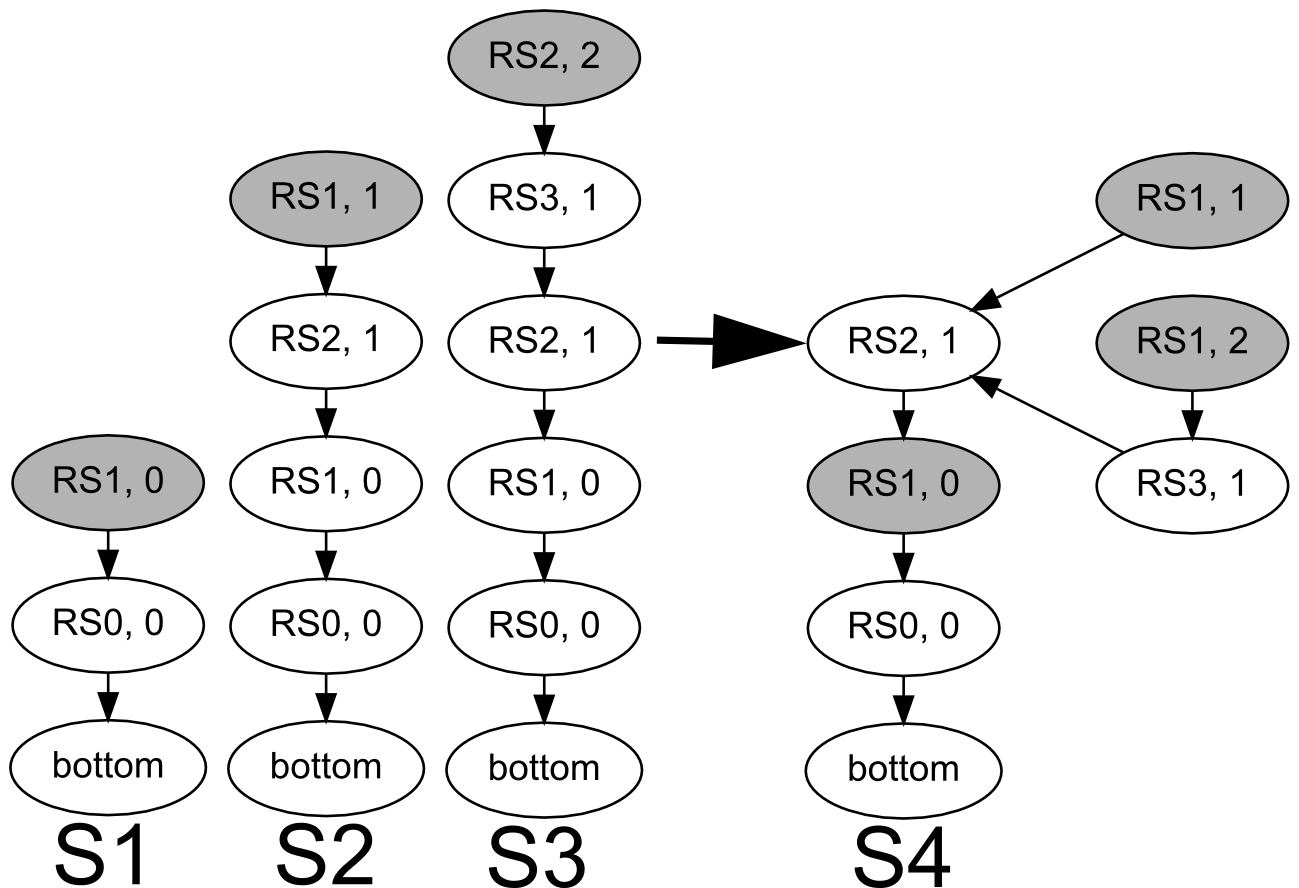
\includegraphics[width=.8\textwidth]{pics/ex_gss.png}
\caption{Пример GSS}
\label{fig:gss} 
\end{center}
\end{figure}

\subsection{Сжатое представление леса разбора}

Для переиспользования общих поддеревьев вывода Ян Рекерс (Jan Rekers, University of Amsterdam) предложил сжатое представление леса разбора (Shared Packed Parse Forest, SPPF)~\cite{SPPF}, которое позволяет компактно представлять множество деревьев вывода. Важным свойством SPPF является то, что из него можно извлечь только те и только те деревья, которые могли быть получены в результате построения вывода конкретного входа в заданной грамматике. Для обеспечения этого свойства в SPPF, кроме терминальных и нетерминальных узлов, добавляются дополнительные узлы различных типов. Конкретный набор типов дополнительные узлов может отличаться в зависимости от алгоритма анализа.

\fvset{frame=lines,framesep=5pt}
\begin{listing}
% * <Екатерина Вербицкая> 17:30:32 02 Jul 2015 UTC+0300:
% Ты вроде вводил правила как нечто со стрелкой, так и выдерживай стиль дальше в тексте.
    \begin{pyglist}[numbers=left,numbersep=5pt]

s ::= m 
s ::= p
p ::= A n
m ::= A l
l ::= n
n ::= B C

\end{pyglist}
\caption{Грамматика $G_1$}
\label{lst:g1}
\end{listing}


Пример SPPF для грамматики $G_1$ (листинг~\ref{lst:g1}) и входа \verb|ABC| приведён на рисунке~\ref{fig:ex_sppf}. Представлены два различных дерева вывода~(\ref{fig:ex_sppf1} и ~\ref{fig:ex_sppf2}) и результат их объединения в SPPF~\ref{fig:ex_sppf3}. Узлы с именами вида ``n <name>'' --- это нетерминальные узлы, ``е <name>'' --- терминальные, ``prod <num>'' --- дополнительные узлы, показывающие, согласно какой продукции из грамматики прозводился вывод нетерминала, являющегося предком данного узла.  

\begin{figure}[h!]
\centering
   \begin{subfigure}[b]{0.3\textwidth}
       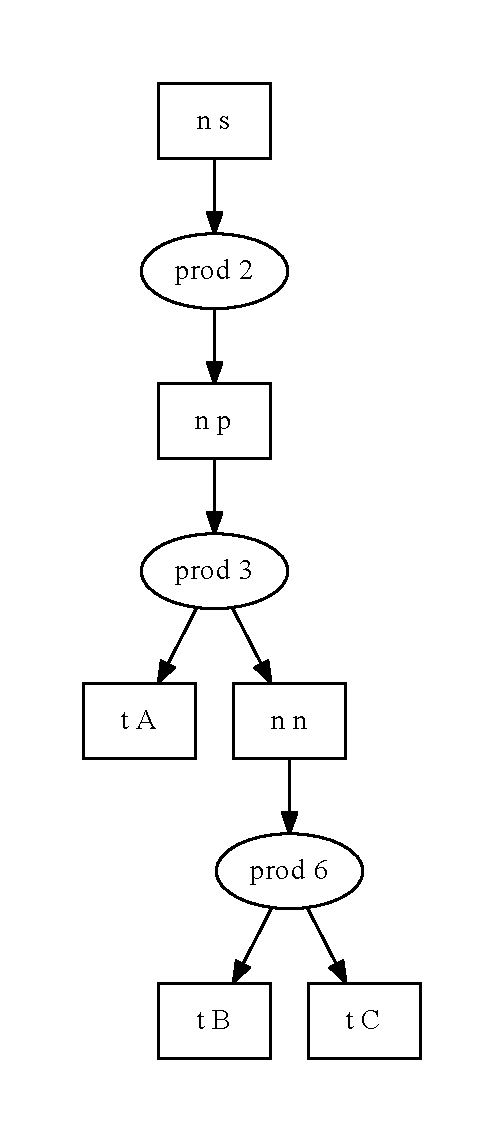
\includegraphics[width=\textwidth]{pics/ex_sppf1}
       \caption{Первое дерево вывода}
       \label{fig:ex_sppf1}
   \end{subfigure}
   ~ 
   \begin{subfigure}[b]{0.3\textwidth}
       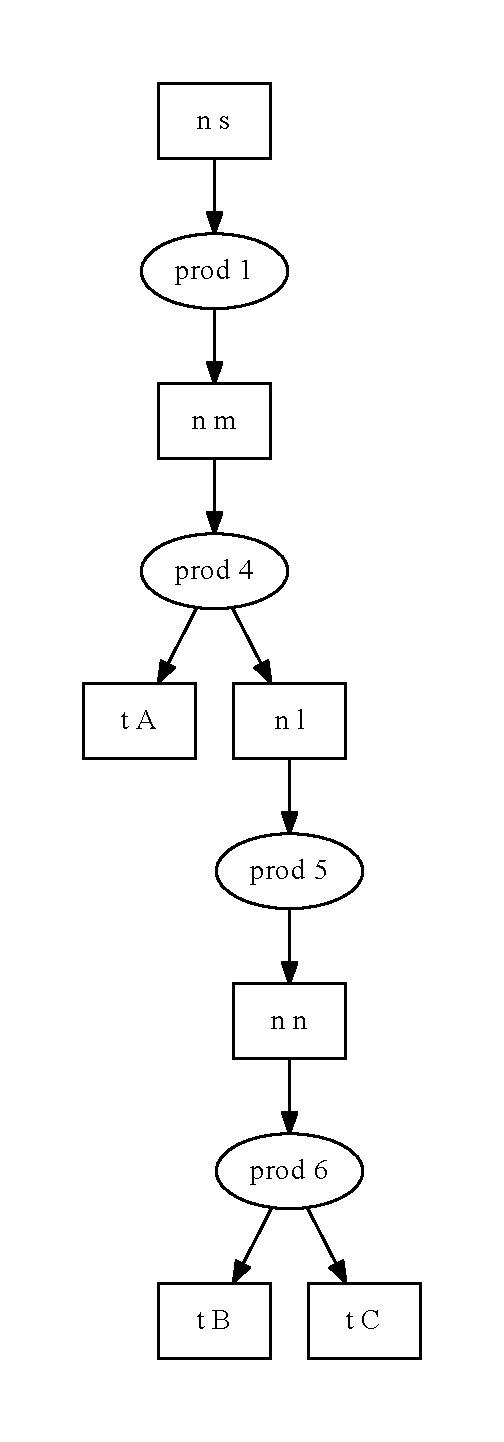
\includegraphics[width=\textwidth]{pics/ex_sppf2}
       \caption{Второе дерево вывода}
       \label{fig:ex_sppf2}
   \end{subfigure}
   ~
   \begin{subfigure}[b]{0.3\textwidth}
       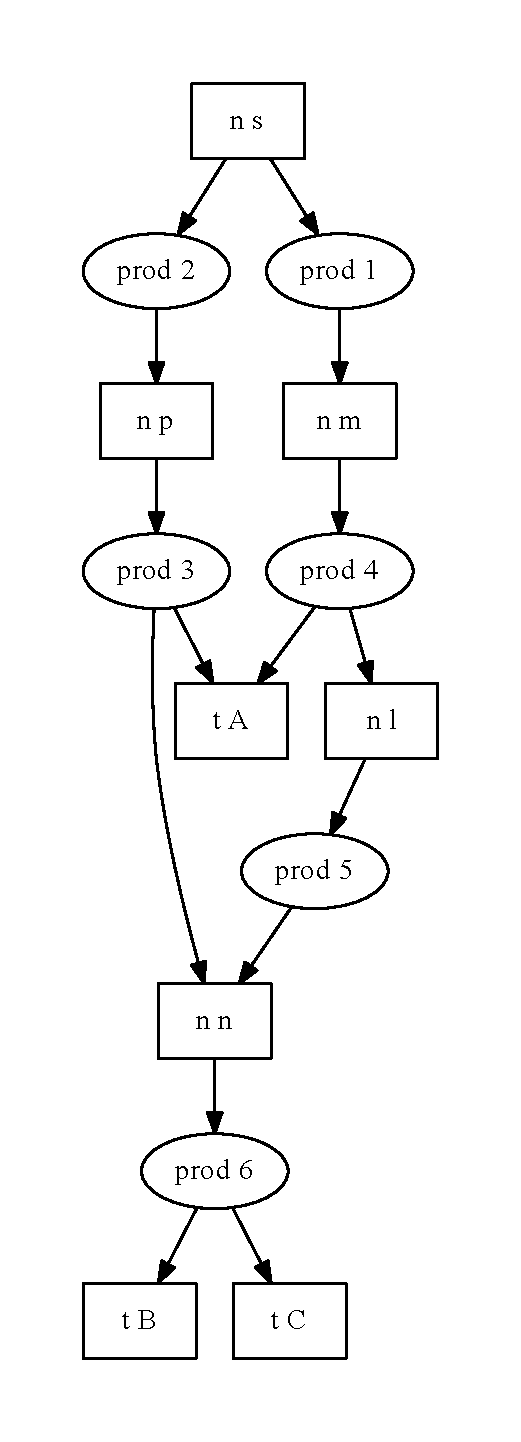
\includegraphics[width=\textwidth]{pics/ex_sppf3}
       \caption{Объединение деревьев вывода в SPPF}
       \label{fig:ex_sppf3}
   \end{subfigure}
   \caption{Пример SPPF для грамматики $G_1$ и входа \textbf{\texttt{ABC}}}
   \label{fig:ex_sppf} 
\end{figure}

\subsection{Алгоритм RNGLR}

RNGLR-алгоритм (Right-Nulled Generalized LR)~\cite{RNGLR} является модификацией предложенного Масару Томитой алгоритма, который не был способен обрабатывать все контекстно-свободные грамматики. Чтобы устранить данный недостаток, Элизабет Скотт (Elizabeth Scott) и Адриан Джонстон (Adrian Johnstone) из университета Royal Holloway (Великобритания) предложили RNGLR-алгоритм, который расширяет GLR-алгоритм специальным способом обработки обнуляемых справа правил (right-nullable rules, имеющих вид $\mathrm{A} \rightarrow \alpha \beta$, где $\beta$ выводит пустую строку $\epsilon$), позволяя обрабатывать произвольные контекстно-свободные грамматики. Алгоритм синтаксического анализа динамически формируемых выражений, представленный в данной работе, основан на RNGLR-алгоритме. Его подробное описание в виде псевдокода приведено ниже.

\begin{listing}[!ht]
\hrule
\begin{algorithmic}[1]
%\caption{RNGLR-алгоритм}
%\label{rnglr}
\Function{parse}{$grammar, input$}
  \State{$\mathcal{R} \gets \emptyset$} \Comment{Очередь троек: вершина GSS, нетерминал, длина свёртки}
  \State{$\mathcal{Q} \gets \emptyset$} \Comment{Коллекция пар: вершина GSS, состояние синтаксического анализатора}
  \If{$input = \epsilon$}
    \If{$grammar$ accepts empty input} {report success}
    \Else { report failure}
    \EndIf
  \Else
    \State{\Call{addVertex}{$0, 0, startState$}}
    \ForAll{$i$ in $0..input.Length-1$}
      \State{\Call{reduce}{$i$}}
      \State{\Call{push}{$i$}}
    \EndFor
    \If{$i=input.Length-1$ and there is a vertex in the last level of GSS which state is accepting}
      \State{report success}
    \Else { report failure}
    \EndIf
  \EndIf
\EndFunction
\Function{reduce}{$i$}
  \While{$\mathcal{R}$ is not empty}
    \State{$(v, N, l) \gets \mathcal{R}.Dequeue()$}
    \State{find the set $\mathcal{X}$ of vertices reachable from $v$ along the path of length $(l-1)$}
    \State{or length $0$ if $l=0$}
    \ForAll{$v_{h} = (level_{h}, state_{h})$ in $\mathcal{X}$}
      \State{$state_{t} \gets$ calculate new state by $state_{h}$ and nonterminal $N$}
      \State{\Call{addEdge}{$i, v_{h}, v.level, state_{tail}, (l=0)$}}
    \EndFor
  \EndWhile
\EndFunction
\Function{push}{$i$}
  \State{$\mathcal{Q^{'}} \gets$ copy $\mathcal{Q}$}
  \While{$\mathcal{Q^{'}}$ is not empty}
    \State{$(v, state) \gets \mathcal{Q}.Dequeue()$}
    \State{\Call{addEdge}{$i, v, v.level + 1, state, false$}}
  \EndWhile
\EndFunction
\end{algorithmic}
\hrule
  \caption{Критерии сравнения инструментов анализа динамически формируемых строковых выражений}\label{lst:metricsForComparison}
\end{listing}

\begin{listing}[!ht]
\hrule

\begin{algorithmic}[1]
\caption{Построение GSS}
\label{RNGLRMain}
\Function{addVertex}{$i, level, state$}
  \If{GSS does not contain vertex $v = (level, state)$}
    \State{add new vertex $v = (level, state)$ to GSS}
    \State{calculate the set of shifts by $v$ and the $input[i+1]$ and add them to $\mathcal{Q}$}
    \State{calculate the set of zero-reductions by $v$ and the $input[i+1]$ and}
    \State{add them to $\mathcal{R}$}
  \EndIf
  \State{\Return{$v$}}
\EndFunction
\Function{addEdge}{$i, v_{h}, level_{t}, state_{t}, isZeroReduction$}
  \State{$v_{t} \gets$ \Call{addVertex}{$i, level_{t}, state_{t}$}}
  \If{GSS does not contain edge from $v_{t}$ to $v_{h}$}
    \State{add new edge from $v_{t}$ to $v_{h}$ to GSS}
    \If{not $isZeroReduction$}
      \State{calculate the set of reductions by $v$ and the $input[i+1]$ and}
      \State{add them to $\mathcal{R}$}
    \EndIf
  \EndIf
\EndFunction
\end{algorithmic}

\hrule
\end{listing}

Для эффективного представления множества стеков во время синтаксического анализа в алгоритме RNGLR, как и в классическом GLR, используется структурированный в виде графа стек (GSS). Вершина GSS~--- это пара $(s,l)$, где $s$~--- состояние синтаксического анализатора, а $l$~--- уровень (позиция во входном потоке).

RNGLR-алгоритм последовательно считывает символы входного потока слева направо, по одному за раз, и строит GSS по ``слоям'': сначала осуществляются все возможные свёртки для данного символа, после чего сдвигается следующий символ со входа. Свёртка или сдвиг модифицируют GSS следующим образом. Предположим, что в GSS необходимо добавить ребро $(v_t,v_h)$. По построению, конечная вершина добавляемой дуги к такому моменту уже обязательно находится в GSS. Если начальная вершина также содержится в GSS, то в граф добавляется новое ребро (если оно ранее не было добавлено), иначе создаются и добавляются в граф и начальная вершина, и ребро. Каждый раз, когда создаётся новая вершина $v=(s,l)$, алгоритм вычисляет новое состояние синтаксического анализатора $s'$ по $s$ и следующему символу входного потока. Пара $(v,s')$, называемая push, добавляется в глобальную коллекцию $\mathcal{Q}$. Также при добавлении новой вершины в GSS вычисляется множество $\epsilon$-свёрток, после чего элементы этого множества добавляются в глобальную очередь $\mathcal{R}$. Свёртки длины $l>0$ вычисляются и добавляются в $\mathcal{R}$ каждый раз, когда создаётся новое (не-$\varepsilon$) ребро. Подробное описание работы со структурированным в виде графа стеком GSS пердставлено в листинге~\ref{RNGLRMain}.

В силу неоднозначности грамматики входная строка может иметь несколько деревьев вывода, как правило, содержащих множество идентичных поддеревьев. Для того, чтобы компактно хранить множество деревьев вывода, используется SPPF, являющееся ориентированным графом и в данном случае обладающее следующей структурой.
\begin{enumerate}
  \item \emph{Корень} соответствует стартовому нетерминалу грамматики.
  \item \emph{Терминальные} вершины, не имеющие исходящих дуг, соответствуют либо терминалам грамматики, либо деревьям вывода пустой строки $\varepsilon$.
  \item \emph{Нетерминальные} вершины являются корнем дерева вывода некоторого нетерминала грамматики; только вершины-продукции могут быть непосредственно достижимы из таких вершин.
  \item \emph{Вершины-продукции}, представляющие правую часть правила грамматики для соответствующего нетерминала. Вершины, непосредственно достижимые из них, упорядочены и могут являться либо терминальными, либо нетерминальными вершинами. Количество таких вершин лежит в промежутке $[l-k \dots l]$, где $l$~--- это длина правой части продукции, а $k$~--- количество финальных символов, выводящих $\varepsilon$. При этом такие символы игнорируются для уменьшения потребления памяти.
\end{enumerate}

SPPF создаётся параллельно с построением GSS. С каждым ребром GSS ассоциирован либо терминальный, либо нетерминальный узел. Когда добавление ребра в GSS происходит во время операции push, новая терминальная вершина создаётся и ассоциируется с ребром. Нетерминальные вершины ассоциируются с рёбрами, добавленными во время операции reduce. Если ребро уже есть в GSS, к ассоциированной с ним нетерминальной вершине добавляется новая вершина-продукция. Подграфы, ассоциированные с рёбрами пути, вдоль которого осуществлялась свёртка, добавляются как дети к вершине-продукции. После того, как входной поток прочитан до конца, производится поиск всех вершин, имеющих принимающее состояние анализатора, после чего подграфы, ассоциированные с исходящими из таких вершин рёбрами, объединяются в один граф. Из полученного графа удаляются все недостижимые из корня вершины, в результате чего остаются только корректные деревья разбора для входной строки. 

Листинг~\ref{rnglr} представляет более детальное описание алгоритма.

    
\section{Используемые инструменты}

В этом разделе описываются основные инструменты, использованные в работе: YaccConstructor~\cite{YCArticle, YCUrl}, выбранный в качастве основы для реализации алгоритма синтаксического анализа динамически формируемых выражений, и ReSharper SDK~\cite{ReSharperSDK}, использованный для разработки сшиений для microsoft Visual Studio IDE.  

\subsection{YaccConstructor}\label{YCDescr}

    Одной из задач данной работы является создание инструментария, упрощающего разработку целевых инструментов статического анализа строковых выражений, которые включают такие этапы, как лексический и синтаксический анализ. При создании лексических и синтаксических анализаторов широко распространённой практикой является использование генераторов, которые по описанию языка строят соответствующий анализатор. Данный подход должен быть реализован и для создания инструментов анализа встроенных языков.
    Работа с описаниями языков программирования --- грамматикой и лексический спецификацией --- в рамках решаемой задачи аналогична работе с ними в стандартных генераторах. По этой причине необходимо было выбрать готовую платформу для работы с грамматиками и создания синтаксических и лексических анализаторов.

        В качестве такой платформы был выбран исследовательский проект лаборатории языковых инструментов JetBrains YaccConstructor (YC)~\cite{YCArticle, YCUrl}, который является модульной платформой с открытым исходным кодом для исследований в области лексического и синтаксического анализа и разработки соответствующих инструментов. YC реализован на платформе Microsoft .NET\footnote{Microsoft .NET --- платформа для разработки программных продуктов компании Microsoft. Общие сведения о платформе: \url{https://msdn.microsoft.com/ru-ru/library/zw4w595w(v=vs.110).aspx} (Посещено 23.06.2015.)}, основной язык разработки --- F\#\footnote{F\# --- функциональный язык программирования для платформы .NET. Информация о языке: \url{http://fsharp.org} (Посещено 23.06.2015.)}~\cite{FSharp}.

\begin{figure}[h!]
\begin{center}
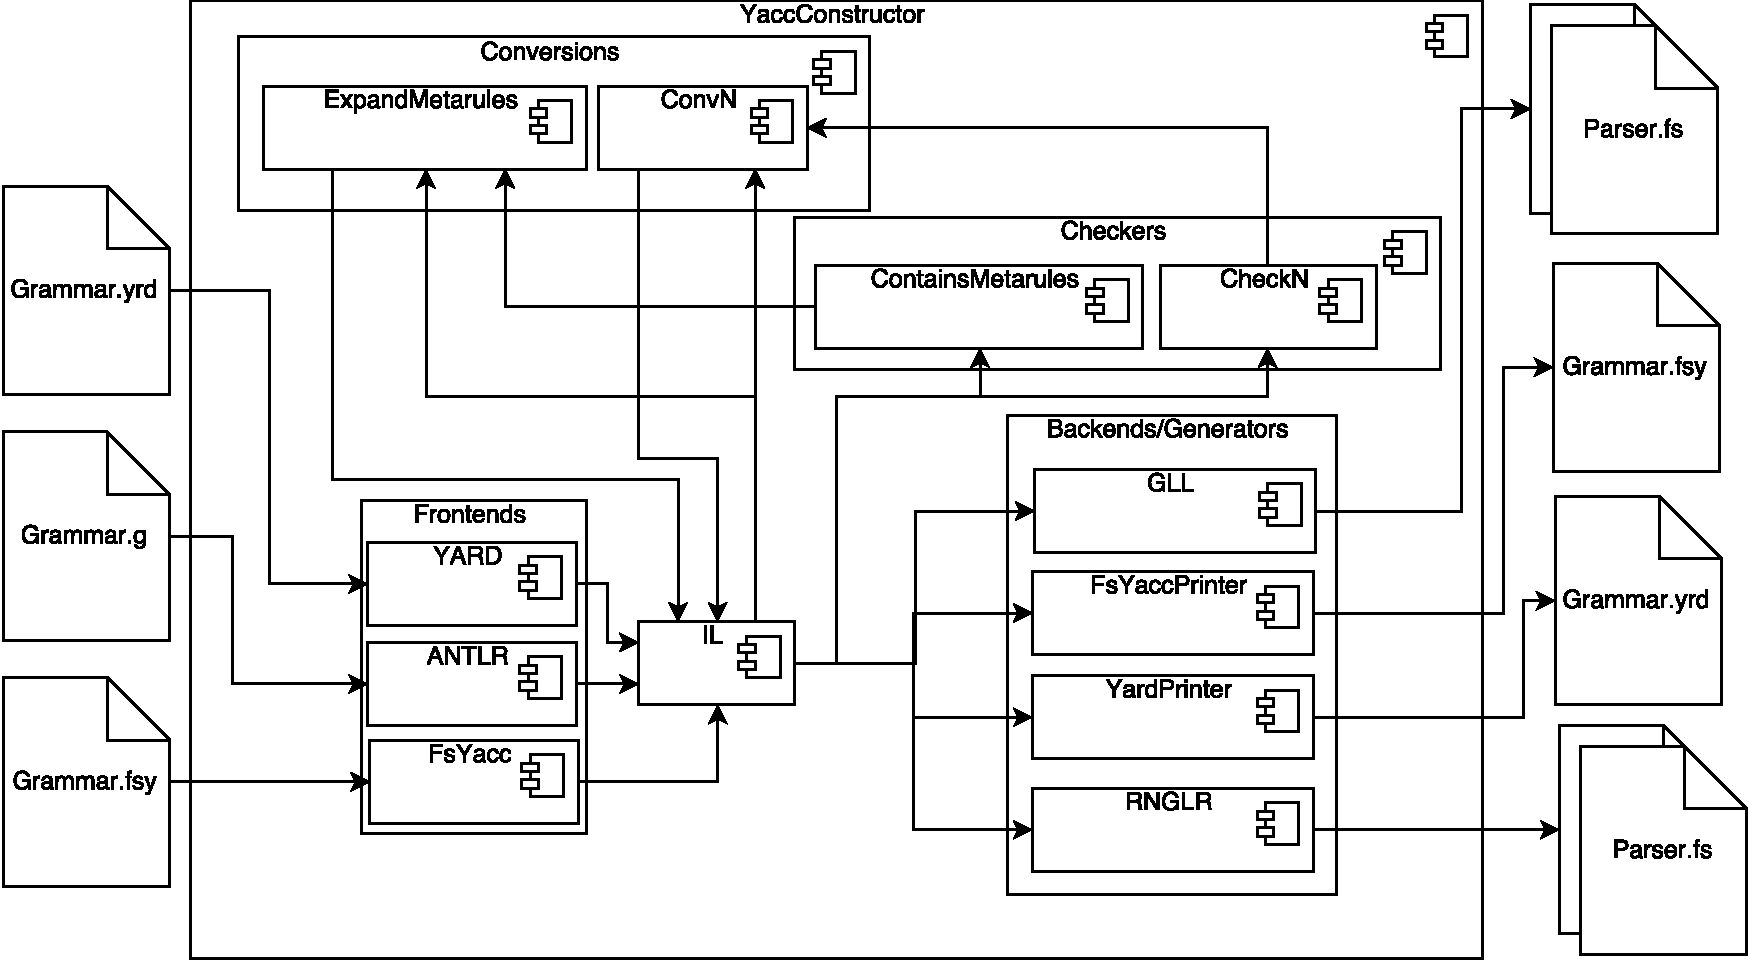
\includegraphics[width=\textwidth]{pics/YCArch.pdf}
\caption{Архитектура платформы YaccConstructor}
\label{fig:ycarch} 
\end{center}
\end{figure}

        
    Архитектура YC, представленная на рисунке~\ref{fig:ycarch}, позволяет собирать требуемый инструмент из существующих модулей: можно выбрать фронтенд, соответствующий используемому языку спецификации грамматики, задать необходимые преобразования грамматики, указать необходимый генератор. Генераторы (backend) представляют различные инструменты, которые по внутреннему представлению грамматики получают результ, полезный для конечного пользователя. Например, это могут быть генераторы синтаксических анализаторов, основанные на различных алгоритмах или принтеры, генерирующие текст грамматики в определённом формате или на заданном языке. YC является расширяемой платформой: модуль любого типа может быть реализован, в том числе с переиспользованием уже существующих, и подключён к платформе.  

    В рамках YC разработан выразительный язык спецификации грамматик YARD, поддерживающий атрибутные грамматики, грамматики в EBNF~\footnote{EBNF --- расфиренная форма Бэкуса-Наура. Грамматики в этой форме позволяют использовать регулярные выражения в правых частях правил~\cite{EBNFISO}.} и многое другое. В листинге~\ref{lst:calcExample} представлена грамматика языка арифметических выражений Calc на языке YARD.  

\fvset{frame=lines,framesep=5pt}
\begin{listing}
    \begin{pyglist}[numbers=left,numbersep=5pt]
    
    [<Start>]
    expr: factor [MULT expr]
    powExpr: NUM | LBR expr RBR
    factor: powExpr [POW factor]
    
\end{pyglist}
\caption{Пример грамматики языка арифметических выражений на языке YARD}
\label{lst:calcExample}
\end{listing}


    Выразительный синтаксис языка описания грамматики удобен для разработчика, однако генераторы, как правило, не поддерживают обработку грамматик в таком виде. Часто требуется, чтобы правая часть правила  грамматики не содержала регулярных выражений, а состояла бы из цепочки из терминалов и нетерминалов. Это необходимо для работы алгоритма построения таблиц. Для решения этой задачи в YC реализован ряд преобразований грамматик. В результате их применения к грамматике, представленной в листинге~\ref{lst:calcExample}, можно получить грамматику, представленную в листинге~\ref{lst:calcTransformExample}.


\fvset{frame=lines,framesep=5pt}
\begin{listing}
    \begin{pyglist}[numbers=left,numbersep=5pt]
    
    [<Start>]
    expr: factor 
    expr: factor MULT expr
    powExpr: NUM 
    powExpr: LBR expr RBR
    factor: powExpr
    factor: powExpr POW factor
    startRule: expr

\end{pyglist}
\caption{Пример преобразованной грамматики языка арифметических выражений}
\label{lst:calcTransformExample}
\end{listing}

    Также в рамках платформы YC в качестве одного из модулей ранее был реализован генератор синтаксических анализаторов на основе RNGLR-алгоритма. Это позволяет переиспользовать общие функции и структуры данных при разработке анализатора для встроенных языков. 
    Таким образом, алгоритм анализа встроенных языков и соответствующий генератор может быть реализован в рамках платформы YC в качестве одного из модулей. При этом можно использовать готовый язык описания грамматики и преобразования, а также переиспользовать необходимые элементы генератора анализаторов на основе RNGLR-алгоритма. Таким образом, YC был выбран в качестве основы для реализации благодаря удобной архитектуре и большому количеству готовых решений. 


\subsection{ReSharper SDK}\label{ReSharperSDKDescr}

    Для демонстрации разработанного в рамках данной работы инструмента представляется целесообразным создать на его основе целевое решение. Для этого необходимо окружение, способное обрабатывать внешний язык, поскольку такие операции над внешним языком, как построение дерева разбора, базовый анализ (например, построение графа потока управления или графа потока данных), лежат за пределами рассматриваемой в данной работе задачи, и их выполнение должно осуществляться сторонними инструментами. При этом такие инструменты должны предоставлять необходимую для решения основной задачи функциональность. Кроме того, необходимо иметь удобный способ взаимодействия с пользователем: необходимо получать код для анализа и отображать результаты в виде, удобном для пользователя. Один из самых распространённых способов работы с программным кодом --- это работа в интегрированной среде разработки.

    Так как реализация работы велась на платформе Microsoft .NET, то соответствующее окружение для обработки внешнего языка и организации взаимодействия с пользователем на данной платформе должно работать на данной платформе. Одной из самых известных сред разработки для платформы .NET, позволяющей создавать расширения на .NET языках, является Microsoft Visual Studio IDE\footnote{Сайт среды разработки Microsoft Visual Studio IDE: \url{https://www.visualstudio.com/} (Посещён 23.06.2015.)}. Она и была выбрана в качестве цели для интеграции инструмента статического анализа строковых выражений. Однако у данной среды разработки достаточно сложный механизм создания расширений, что вызвано его универсальностью. При решении нашей задачи универсальность не требовалась, поэтому можно было бы использовать менее универсальный и более простой механизм.

Такой механизм предоставляется ReSharper SDK~\cite{ReSharperSDK}.  ReSharper~\cite{ReSharper} --- расширение для Microsoft Visual Studio, предоставляющее пользователю широкий набор дополнительных анализов кода. Для разработчиков предоставляется свободно распространяемая SDK, реализующая анализ таких языков, как C\#, VB.NET и др. Большая часть функциональности ReSharper выделена в свободно распространяемую SDK, что даёт возможность сторонним разработчикам создавать собственные расширения к ReSharper, переиспользуя его функциональность. В контексте данной работы это позволяет упростить создание плагинов для поддержки различных встроенных языков. Кроме того, ReSharper SDK предоставляет более удобную ``обёртку'' над многими интерфейсами Microsoft Visual Studio, что упрощает взаимодействие с ней и полезно, например, при предоставлении результатов пользователю.

Следует также отметить, что ReSharper является многоязыковым инструментом, то есть поддерживает большой набор различных языков и спроектирован так, чтобы максимально упростить поддержку новых языков. Это позволяет создавать инструменты, обрабатывающие не только различные встроенные языки, но также и различные внешние.

 Выделим следующую функциональность ReSharper SDK, необходимую для реализации поддержки встроенных языков в Microsoft Visual Studio.  
\begin{itemize}
    \item Построение дерева разбора внешнего языка (C\#, JavaScript и другие, поддерживаемые ReSharper), узлы которого содержат координаты в исходном коде, что позволяет точно связывать текстовое и структурное представление кода.
    \item Анализ потока данных и анализ потока управления для поддерживаемых языков. На основе существующих анализов можно строить более сложные, необходимые, например, для построения регулярной аппроксимации.
    \item Вывод сообщений об ошибках и графическое выделение некорректных мест в текстовом редакторе.
    \item Взаимодействие с редактором кода, позволяющее настраивать подсветку синтаксиса, получать позицию курсора и управлять ею, что нужно для динамической подсветки парных элементов.
\end{itemize}

Таким образом ReSharper SDK и Microsoft Visual Studio IDE выбраны в качестве основы для разработки целевого инструмента на основе представленных в данной работе результатов.

\section{Выводы}

На основе проведённого обзора можно сделать следующие выводы, обосновывающие необходимость проведения исследований в области статического анализа динамически формируемых строковых выражений.

\begin{itemize}
    \item Проблема анализа строковых выражений актуальна в нескольких областях: поддержка встроенных языков в интегрированных средах разработки, оценка качества кода, содержащего динамически формируемые строковые выражения, реинжиниринг программного обеспечения.
    \item Большинство реализаций поддерживают конкретный внешний и конкретный встроенный язык и, как правило, решают одну достаточно узкую задачу. При этом, зачастую, плохо расширяемы, как в смысле поддержки других языков, так и в смысле решения новых задач. Полноценные средства разработки инструментов статического анализа динамически формируемых выражений, упрощающие создание решений для новых языков, отсутствуют.
    \item Для эффективного решения этих задач необходимо структурное представление кода, однако на текущий момент не представлено законченного решения, позволяющего строить деревья вывода для динамически формируемых выражений.
\end{itemize}

Кроме того, обзор позволяет выявить следующие подходы, технологии и средства.

\begin{itemize}
    \item В качестве приближения множества значений целесообразно использовать регулярную аппроксимацию~\cite{JSA, RegOverApprox}, так как при работе с ней ряд важных задач является разрешимым в общем случае, что не верно для контекстно-свободной. Более того, работа с регулярной аппроксимацией упрощает решение такой задачи, как лексический анализ встроенных языков.
    \item Лексический и синтаксический анализы должны быть разделены. Это оправдано как с теоретической, так и с практической точек зрения, так как лексический анализ не привносит потери точности и упрощается переиспользование спецификаций языков и самих анализаторов. 
    \item В качестве основы алгоритма синтаксического анализа днамически формируемых выражений можно выбрать алгоритм обобщённого синтаксического анализа~\cite{GeneralisedlrBIG}, так как в нём реализовано эффективное управление множеством стеков и деревьев разбора, что важно при работе с динамически формируемыми выражениями.
\end{itemize}
\clearpage

\section{Relaxed Parsing of Regular Sets}

The input of the algorithm (see Algorithm~\ref{parsing}) is a reference grammar $G$ with alphabet of terminal symbols $T$ 
and a finite non-deterministic automaton $(Q, \Sigma, \delta, q_0, q_f)$ with a single start state $q_0$, single final state $q_f$ 
and no $\epsilon$-transitions, where $\Sigma \subseteq T$~--- alphabet of input symbols, $Q$~--- alphabet of states, 
$\delta$~--- transition relation. RNGLR parser tables and some accessory information (called $parserSource$ in pseudocode) 
are generated for the grammar $G$. 

The general idea of the algorithm is to traverse the automaton graph and sequentially construct GSS, similarly to RNGLR.
However, as we deal with a graph instead of a linear stream, the next symbol turns into the \emph{set of terminals} on the 
all outgoing edges of current vertex. This results in a a different semantics of pushing and reducing (see line~5, 
Algorithm~\ref{processVertex}, and lines~8 and~20, Algorithm~\ref{gss_construction}). We use queue $\mathcal Q$ to control the 
order of automaton graph vertices processing. Every time a new GSS vertex is added, all zero-reductions have to be performed 
and then new tokens have to be shifted, so a corresponging graph vertex has to be enqueueed for further processing. 
Addition of new GSS edge can produce reductions to handle, so the graph vertex at the tail of the added edge has 
also to be enqueueed (see Algorithm~\ref{gss_construction}). Reductions are applied along the paths in GSS, and if we add
a new edge to some tail vertex, which was already presented in GSS, we also have to recalculate all \emph{passing} reductions
(see \emph{applyPassingReductions} function in Algorithm~\ref{processVertex}).

Likewise RNGLR, we associate GSS vertices with positions in the input,
and, in our case, a position coinsides with some state of the input automaton. We construct some
inner data structure (referred to as inner graph) by copying input automaton graph and 
extending each its vertex with the following collections: 

\begin{itemize}
  \item \emph{processed}: GSS vertices, for which all the pushes were processed. 
   This set aggregates all GSS vertices, associated with inner graph vertex.
  \item \emph{unprocessed}: GSS vertices, for which all the pushes are to be processed. 
   This set is analogous to $\mathcal{Q}$ of original RNGLR.
  \item \emph{reductions}: a queue, which is analogous to $\mathcal{R}$ of original RNGLR: 
   all reductions to be processed.
  \item \emph{passingReductionsToHandle}: pairs of GSS vertex and GSS edge to apply 
   passing reductions along them.
\end{itemize}

Besides parser $state$ and $level$ (which is equal to the input automaton state), 
a collection of \emph{passing reductions} is stored in a GSS vertex. Passing reduction is a 
triplet $(startV, N, l)$, representing reductions, whose path contains given GSS vertex. 
This triplet is similar to one describing reduction, where $l$ is a remaining length of the path. 
Passing reductions are stored for every vertex of the path (except for the first and the last) 
during path search in \emph{makeReductions} function (see Algorithm~\ref{processVertex}).

We inherit SPPF construction from the original RNGLR; in our case, 
derivation trees for strings, accumulated along the paths of the input automaton 
graph, are merged. 

\begin{algorithm}[!ht]
\begin{algorithmic}[1]
\caption{Parsing algorithm}
\label{parsing}
\Function{parse}{$grammar, automaton$}
  \State{$inputGraph \gets$ construct inner graph representation of $automaton$}
  \State{$parserSource \gets$ generate RNGLR parser tables for $grammar$}
  \If{$inputGraph$ contains no edges}
    \If{$parserSource$ accepts empty input} {report success}
    \Else { report failure}
    \EndIf
  \Else
    \State{\Call{addVertex}{$inputGraph.startVertex, startState$}}
    \State{$\mathcal{Q}.Enqueue(inputGraph.startVertex)$}
    \While{$Q$ is not empty}
      \State{$v \gets \mathcal{Q}.Dequeue()$}
      \State{\Call{makeReductions}{$v$}}
      \State{\Call{push}{$v$}}
      \State{\Call{applyPassingReductions}{$v$}}
    \EndWhile
    \If{$v_f.level = q_f$ and $v_f.state$ is accepting} {report success}
    \Else { report failure}
    \EndIf
  \EndIf
\EndFunction
\end{algorithmic}
\end{algorithm}

\begin{algorithm}[!ht]
\begin{algorithmic}[1]
\caption{Single-vertex processing}
\label{processVertex}
\Function{push}{$innerGraphV$}
  \State{$\mathcal{U} \gets$ copy $innerGraphV.unprocessed$}
  \State{clear $innerGraphV.unprocessed$}
  \ForAll{$v_{h}$ in $\mathcal{U}$}  
    \ForAll{$e$ in outgoing edges of $innerGraphV$}
      \State{$push \gets$ calculate next state by $v_{h}.state$ and the token on $e$}
      \State{\Call{addEdge}{$v_{h}, e.Target, push, false$}}
      \State{add $v_{h}$ in $innerGraphV.processed$}
    \EndFor
  \EndFor
\EndFunction

\Function{makeReductions}{$innerGraphV$}
  \While{$innerGraphV.reductions$ is not empty}
    \State{$(startV, N, l) \gets innerGraphV.reductions.Dequeue()$}
    \State{find the set of vertices $\mathcal{X}$ reachable from $startV$}
    \State{along the path of length ($l-1$), or $0$ if $l=0$;}
    \State{add $(startV, N, l-i)$ in $v.passingReductions$,}
    \State{where $v$ is an $i$-th vertex of the path}
    \ForAll{$v_{h}$ in $\mathcal{X}$}
      \State{$state_{t} \gets$ calculate new state by $v_{h}.state$ and nonterminal $N$}
      \State{\Call{addEdge}{$v_{h}, startV, state_{t}, (l=0)$}}
    \EndFor
  \EndWhile
\EndFunction

\Function{applyPassingReductions}{$innerGraphV$}
  \ForAll{$(v, edge)$ in $innerGraphV.passingReductionsToHandle$}
    \ForAll{$(startV, N, l) \gets v.passingReductions.Dequeue()$}
      \State{find the set of vertices $\mathcal{X}$,}
      \State{reachable from $edge$ along the path of length ($l-1$)}
      \ForAll{$v_{h}$ in $\mathcal{X}$}
        \State{$state_{t} \gets$ calculate new state by $v_{h}.state$ and nonterminal $N$}
        \State{\Call{addEdge}{$v_{h}, startV, state_{t}, false$}}
      \EndFor
    \EndFor
  \EndFor
\EndFunction
\end{algorithmic}
\end{algorithm}
 
\begin{algorithm}[!ht]
\begin{algorithmic}[1]
\caption{GSS construction}
\label{gss_construction}
\Function{addVertex}{$innerGraphV, state$}
  \If{$innerGraphV.processed$ or $innerGraphV.unprocessed$ contains\\
    vertex $v$ with state = $state$ }
    \State{\Return{($v, false$)}}
  \Else
    \State{$v \gets$ create new vertex for $innerGraphV$ with state $state$}
    \State{add $v$ in $innerGraphV.unprocessed$}
    \ForAll{$e$ in outgoing edges of $innerGraphV$}
      \State{calculate the set of zero-reductions by $v$}
      \State{and the token on $e$ and add them in $innerGraphV.reductions$}
    \EndFor
    \State{\Return{$(v, true$)}}
  \EndIf
\EndFunction

\Function{addEdge}{$v_{h}, innerGraphV, state_{t}, isZeroReduction$}
  \State{$(v_{t}, isNew) \gets$ \Call{addVertex}{$innerGraphV, state_{t}$}}
  \If{GSS does not contain edge from $v_{t}$ to $v_{h}$}
    \State{$edge \gets$ create new edge from $v_{t}$ to $v_{h}$}
    \State{$\mathcal{Q}.Enqueue(innerGraphV)$}
    \If{not $isNew$ and $v_{t}.passingReductions.Count>0$}
      \State{add $(v_{t}, edge)$ in $innerGraphV.passingReductionsToHandle$}
    \EndIf
    \If{not $isZeroReduction$}
      \ForAll{$e$ in outgoing edges of $innerGraphV$}
        \State{calculate the set of reductions by $v$}
        \State{and the token on $e$ and add them in $innerGraphV.reductions$}
      \EndFor
    \EndIf
  \EndIf
\EndFunction
\end{algorithmic}
\end{algorithm}

We conclude this section by justification of termination and correctness of our algorithm.

\textsc{Theorem 1.}
\textit{Algorithm terminates for any input.}

\textsc{Proof.}
Each vertex of inner representation of the input finite automaton contains, at most, 
$N$ GSS vertices, where $N$ is a number of parser states. So, the total number of 
GSS vertices is, at most, $N\times n$, where $n$ is the number of vertices in the inner graph. 
Since GSS has no multi-edges, the number of its edges is $O((N\times n)^2)$. The algorithm 
dequeues vertex to be processed from $\mathcal Q$ in the each iteration of the 
main loop. Vertices are enqueued to $\mathcal Q$ only when a new edge is added to GSS. Since the number of 
GSS edges is finite, the algorithm always terminates. \qed

To prove correctness, we first introduce the following definition:

\textsc{Definition.} 
\emph{Correct tree} is an ordered tree with the following properties:
\begin{enumerate}
  \item The root is the start nonterminal of the grammar $G$.
  \item The leaf nodes are terminals of $G$. The sequence of the leaf nodes 
        corresponds to some path in the inner graph. 
  \item The interior nodes are nonterminals of $G$. All children of nonterminal 
        $N$ correspond to the symbols of the right-hand side of some production for $N$ in $G$.
\end{enumerate}

Informally, correct tree is a derivation tree (w.r.t reference grammar) for some word in 
the regular approximation. Now we have to prove, that SPPF contains only correct trees.

\textsc{Lemma.}
For every GSS edge $(v_{t}, v_{h})$, $v_{t} \in V_{t}.processed$, $v_{h} \in V_{h}.processed$, 
the terminals of the associated subtree correspond to some path in the inner graph $p$ 
from $V_{h}$ to $V_{t}$.

\textsc{Proof.}
The proof is by induction on the height of derivation tree. 
The base case is either some $\epsilon$-tree or a tree with the single leaf. An $\epsilon$-tree corresponds 
to a path of zero length; the tail and the head of the edge associated with $\epsilon$-tree are identical, 
thus the statement is true. A tree with the single leaf corresponds to a single terminal read from an edge 
($V_{h}$, $V_{t}$) of the inner graph, thus the statement is true.

A tree of height $k$ has a nonterminal $N$ as its root. By third statement of correct tree definition, 
there is a production $N \rightarrow A_{0}, A_{1}, \dots, A_{n}$ for children $A_{0}, A_{1}, \dots, A_{n}$ of the root node. 
A subtree $A_{i}$ is associated with GSS edge $(v_{t}^{i}, v_{h}^{i})$ and, as its height is $k-1$, by inductive hypothesis,
there is a path in the inner graph from $V_{h}^{i}$ to $V_{t}^{i}$. $V_{t}^i = V_{h}^{i+1}$, since $v_{t}^i = v_{h}^{i+1}$, 
thus there is a path in the inner graph from $V_{h}^{0}$ to $V_{t}^{n}$, corresponding to the tree under consideration.
\qed

\textsc{Theorem 2.} 
\textit{Every generated from SPPF tree is correct.}

\textsc{Proof.} Consider arbitrary tree, generated from SPPF, and prove that it is correct. The first and the third statements
of correctness definition immediately follow from SPPF definition. 

{\bf (did'not understand the following statement; Russian decryption is required:)}
\textsc{Lemma 1} proves the second item of the definition by consideration of all the edges from the GSS vertex
on the last level having accepting state to the vertex on the 0-level with the start parser state.

\qed

\textsc{Theorem 3.} 
\textit{For every path $p$ in the inner graph, a correct tree corresponding to $p$ can be generated from SPPF.}

\textsc{Proof.}
Consider arbitrary correct tree and show it can be generated from SPPF. The proof follows the proof of correctness 
for RNGLR-algorithm, except the following moment. RNGLR constructs GSS layer-by-layer: it is guaranteed, that $j$-th 
level of the GSS $\forall j \in [0..i-1]$ would be fixed by the time, when $i$-th level is processed. In our case, 
this property does not hold, which leads to possible generation of the paths for reductions already applied. 
The only possible way to actually add a new path is to add an edge $(v_{t}, v_{h})$, where $v_{t}$ is already in the GSS and 
it has incoming edges. Since the algorithm stores, which reductions have passed through each vertex, it is sufficient to 
{\bf (what does it mean: ``continue passing reductions?'')} continue passing reductions, stored in $v_{t}$ to overcome this problem, 
and this is exactly what \emph{applyPassingReductions} function does. 
\qed

\section{Доказательство корректности алгоритма}

\begin{theorem}{Завершаемость.}
	Алгоритм завершает работу за конечное число шагов для произвольных входных данных
\end{theorem}

\begin{theorem}{Корректность.}
	???
\end{theorem}
\section{Evaluation}

We evaluate the implemented algorithm on both regular and context-free path queries in order to demonstrate applicability of the proposed solution.
Namely, goals of the evaluation are following.
\begin{enumerate}
	\item Investigate the practical applicability of RPQ evaluation by the proposed algorithm.
	\item Compare Azimov's algorithm for reachability CFPQ and the proposed algorithm.
	\item Investigate the practical applicability of paths extraction algorithm for both regular and context-free queries.
\end{enumerate}

For evaluation, we use a PC with Ubuntu 18.04 installed.
It has Intel core i7-6700 CPU, 3.4GHz, and DDR4 64Gb RAM.
As far as we evaluate only algorithm execution time, we store each graph fully in RAM as its adjacency matrix in sparse format.
Note, that graph loading time is not included in the result time of evaluation.	

\subsection{RPQ Evaluation}

In oder to investigate applicability of the proposed algorithm for RPQ over real-world graphs we collect a set of real-world and synthetic graphs and evaluate queries generated by using the most popular templates for RPQs.

\subsubsection{Dataset}

Brief description of collected graphs are presented in Table~\ref{tbl:graphs_for_rpq}.
Namely, the dataset consists of several parts.
The first one is a set of LUBM graphs\footnote{Lehigh University Benchmark (LUBM) web page: \url{http://swat.cse.lehigh.edu/projects/lubm/}. Access date: 07.07.2020.}~\cite{10.1016/j.websem.2005.06.005} with a different number of vertices.
The second one is a graphs from Uniprot database\footnote{Universal Protein Resource (UniProt) web page: \url{https://www.uniprot.org/}. All files used for evaluation can be downloaded here: \url{ftp://ftp.uniprot.org/pub/databases/uniprot/current_release/rdf/}. Access date: 07.07.2020.}: \textit{proteomes}, \textit{taxonomy} and \textit{uniprotkb}.
The last part is a RDF files \textit{mappingbased\_properties} from DBpedia\footnote{DBpedia project web site: \url{https://wiki.dbpedia.org/}. Access date: 07.07.2020.} and \textit{geospecies}\footnote{The Geospecies RDF: \url{https://old.datahub.io/dataset/geospecies}. Access date: 07.07.2020.}.
These graphs represent data from different areas and they are frequently used for graph querying algorithms evaluation.

\begin{table}
{
\rowcolors{2}{black!2}{black!10}
\begin{tabular}{|l|c|c|}
\hline
Graph & \#V & \#E \\
\hline
\hline 
LUBM1k  & 120 926 & 484 646 \\
LUBM3.5k  & 358 434 & 144 9711 \\
LUBM5.9k  & 596 760 & 2 416 513 \\
LUBM1M   & 1 188 340 & 4 820 728 \\
LUBM1.7M & 1 780 956 & 7 228 358 \\
LUBM2.3M & 2 308 385 & 9 369 511 \\
\hline
Uniprotkb & 6 442 630 & 24 465 430 \\
Proteomes & 4 834 262 & 12 366 973 \\
Taxonomy & 5 728 398 & 14 922 125 \\
\hline
Geospecies & 450 609 & 2 201 532 \\
Mappingbased\_properties & 8 332 233 & 25 346 359 \\
\hline
\end{tabular}
}
\caption{Graphs for RPQ evaluation}
\label{tbl:graphs_for_rpq}
\end{table}


Queries for evaluation was generated by using templates of the most popular RPQs which are collected from~
\cite{Pacaci2020RegularPQ} (Table 2) and~\cite{Wang2019} (some of complex queries from Table 5), and are presented in table~\ref{tbl:queries_templates}.
We generate 10 queries for each template and each graph using the most frequent relations from the given graph randomly\footnote{Used generator is available as part of CFPQ\_data project: \url{https://github.com/JetBrains-Research/CFPQ_Data/blob/master/tools/gen_RPQ/gen.py}. Access data: 07.07.2020.}. 
For all LUBM graphs common set of queries was generated in order to investigate scalability of the proposed algorithm.

\begin{table}
{\small
\renewcommand{\arraystretch}{1.25}
\rowcolors{2}{black!2}{black!10}
\begin{tabular}{|c|c||c|c|}
\hline

Name & Query & Name & Query \\
\hline
\hline 
$Q_1$   & $a^*$                               & $Q_9^5$    & $(a \mid b \mid c \mid d \mid e)^+$                     \\
$Q_2$   & $a\cdot b^*$                        & $Q_{10}^2$ & $(a \mid b) \cdot c^*$                                  \\
$Q_3$   & $a \cdot b^* \cdot c^*$             & $Q_{10}^3$ & $(a \mid b \mid c)  \cdot d^*$                          \\
$Q_4^2$ & $(a \mid b)^*$                      & $Q_{10}^4$ & $(a \mid b \mid c \mid d)  \cdot e^*$                   \\
$Q_4^3$ & $(a \mid b \mid c)^*$               & $Q_{10}^5$ & $(a \mid b \mid c \mid d \mid e)  \cdot f^*$            \\
$Q_4^4$ & $(a \mid b \mid c \mid d)^*$        & $Q_{10}^2$ & $a \cdot b$                                             \\
$Q_4^5$ & $(a \mid b \mid c \mid d \mid e)^*$ & $Q_{11}^3$ & $a \cdot b \cdot c$                                     \\
$Q_5$   & $a \cdot b^* \cdot c$               & $Q_{11}^4$ & $a \cdot b \cdot c \cdot d$                             \\
$Q_6$   & $a^* \cdot b^*$                     & $Q_{11}^5$ & $a \cdot b \cdot c \cdot d \cdot f$                     \\
$Q_7$   & $a \cdot b \cdot c^*$               & $Q_{12}$   & $(a \cdot b)^+ \mid  (c \cdot d)^+$                     \\
$Q_8$   & $a? \cdot b^*$                      & $Q_{13}$   & $(a \cdot(b \cdot c)^*)^+ \mid  (d \cdot f)^+$          \\
$Q_9^2$ & $(a \mid b)^+$                      & $Q_{14}$   & $(a \cdot b \cdot (c \cdot d)^*)^+  \cdot (e \mid f)^*$ \\
$Q_9^3$ & $(a \mid b \mid c)^+$               & $Q_{15}$   & $(a \mid b)^+ \cdot (c \mid d)^+$                       \\
$Q_9^4$ & $(a \mid b \mid c \mid d)^+$        & $Q_{16}$   & $a \cdot b \cdot (c \mid d \mid e)$                     \\
\hline
\end{tabular}
}
\caption{Queries' templates for RPQ evaluation}
\label{tbl:queries_templates}
\end{table}


\subsubsection{Results}

For reachability index creation average time of 5 runs is presented.

Reachability index creation time for each query for LUBM graphs set is presented in figure~\ref{fig:lubm_all_qs}.
We can observe linear !!!! dependency of evaluation time on graph size.
Also we can see, that query evaluation time depends on query: there are queries which evaluate less then 1 second even for biggest graph ($Q_2$, $Q_5$, $Q_{11}^2$, $Q_{11}^3$), while worst time is 6.26 seconds ($Q_{14}$).
Anyway, we can argue that in this case our algorithm demonstrates reasonable time to be applied for real-world data analysis, because it is comparable with recent results on the same problem for LUBM querying by using distributed system over 10 nodes~\cite{Wang2019}, while we use only one node. 
Note, that accurate comparison of different approaches is a huge interesting work for the future.

\begin{figure}
   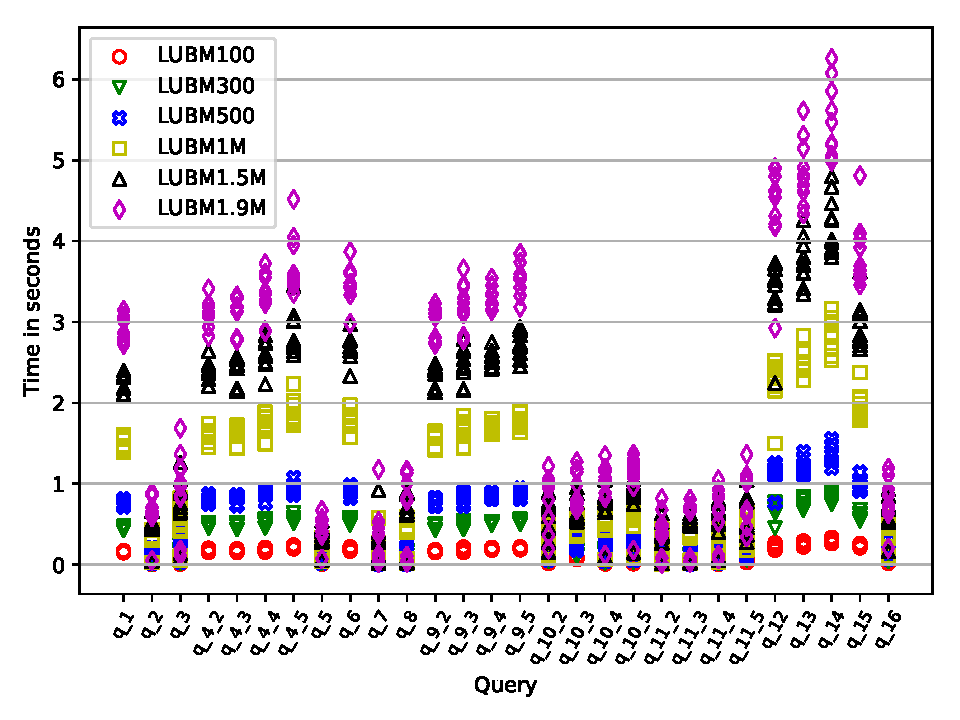
\includegraphics[width=0.48\textwidth]{data/LUBM_all.pdf}
   \caption{Reachability index creation time for LUBM graphs}
   \label{fig:lubm_all_qs}
\end{figure}

Reachability index creation time for each query for for real-world graphs is presented in figure~\ref{fig:other_all_qs}.
We can see that query evaluation time depends on graph inner structure. 
First of all, in some cases handling of small graph requires more time, then handling bigger graph.
For example, $Q_{10}^4$: querying the \textit{geospecies} graph (450k vertices) in some cases requires more time than querying of \textit{mappingbased\_properties} (8.3M vertices) and \textit{taxonomy} (5.7M vertices).
On the other hand, \textit{taxonomy} querying in relatively big number of cases requires significantly more time, than querying of other graphs, while \textit{taxonomy} is not a biggest graph. 
Finally, we can see, that in big number of cases query execution time requires less then 10 seconds, even for big graph, and no queries which require more then 52.17 seconds. 

\begin{figure}
   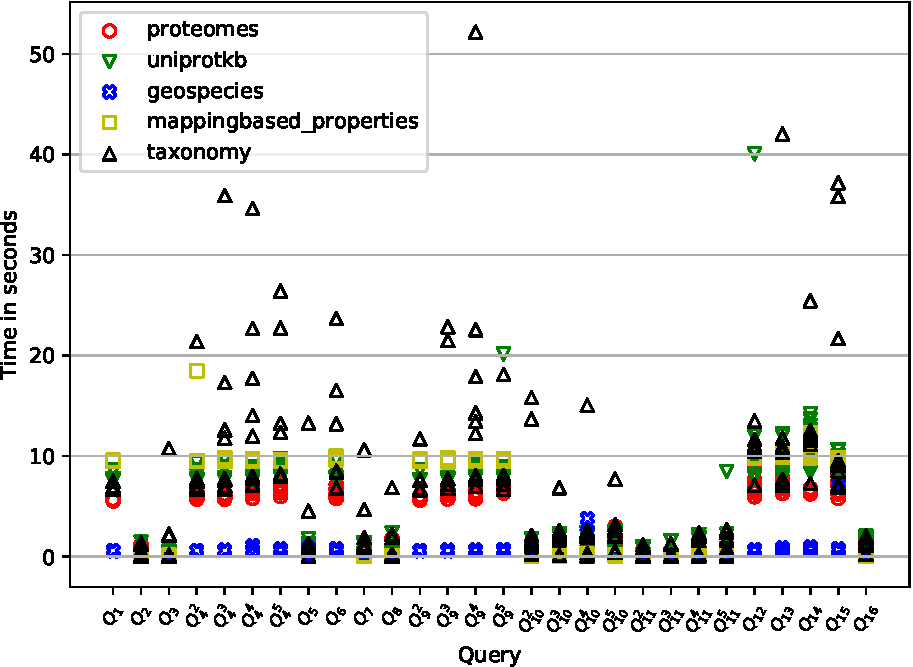
\includegraphics[width=0.48\textwidth]{data/other_all.pdf}
   \caption{Reachability index creation time for real-world RDFs}
   \label{fig:other_all_qs}
\end{figure}

Paths extraction was evaluated on cases with possible long paths.
These cases were selected during reachability index creation by using number of iterations in transitive closure evaluation.
For each selected graph and query we measure paths extraction time for each reachable pair, reachability index creation time is not included because exactly the same index, as calculated at the previous step, is used for paths extraction. 

We evaluate two scenarios.
The first one is a single path extraction.
In this case results are represented as a dependency of extraction time on extracted path length.
We can see linear !!!!

The second scenario is many paths extraction.
Here we limit a number of path to extract by !!! 
In this case results are represented as a dependency of extraction time on number of extracted paths.


\begin{figure}
     \begin{subfigure}[b]{0.24\textwidth}
         \centering
         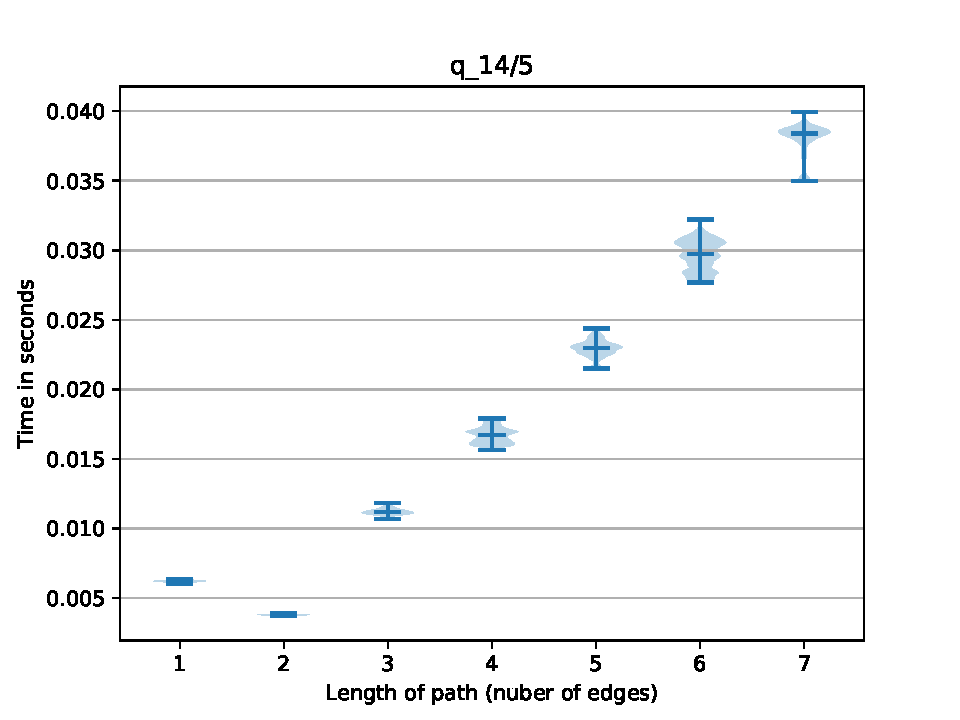
\includegraphics[width=\textwidth]{data/res_graphics/q_14_5.pdf}
         \caption{$y=x$}
         \label{fig:y equals x}
     \end{subfigure}
     ~\begin{subfigure}[b]{0.24\textwidth}
         \centering
         %\includegraphics[width=\textwidth]{data/res_graphics/q9_2_8.pdf}
         \caption{$y=x$}
         \label{fig:y equals x}
     \end{subfigure}\\
     \begin{subfigure}[b]{0.24\textwidth}
         \centering
         %\includegraphics[width=\textwidth]{data/res_graphics/q_14_8.pdf}
         \caption{$y=x$}
         \label{fig:y equals x}
     \end{subfigure}
     ~\begin{subfigure}[b]{0.24\textwidth}
         \centering
         %\includegraphics[width=\textwidth]{data/res_graphics/q4_2_8.pdf}
         \caption{$y=x$}
         \label{fig:y equals x}
     \end{subfigure}
   %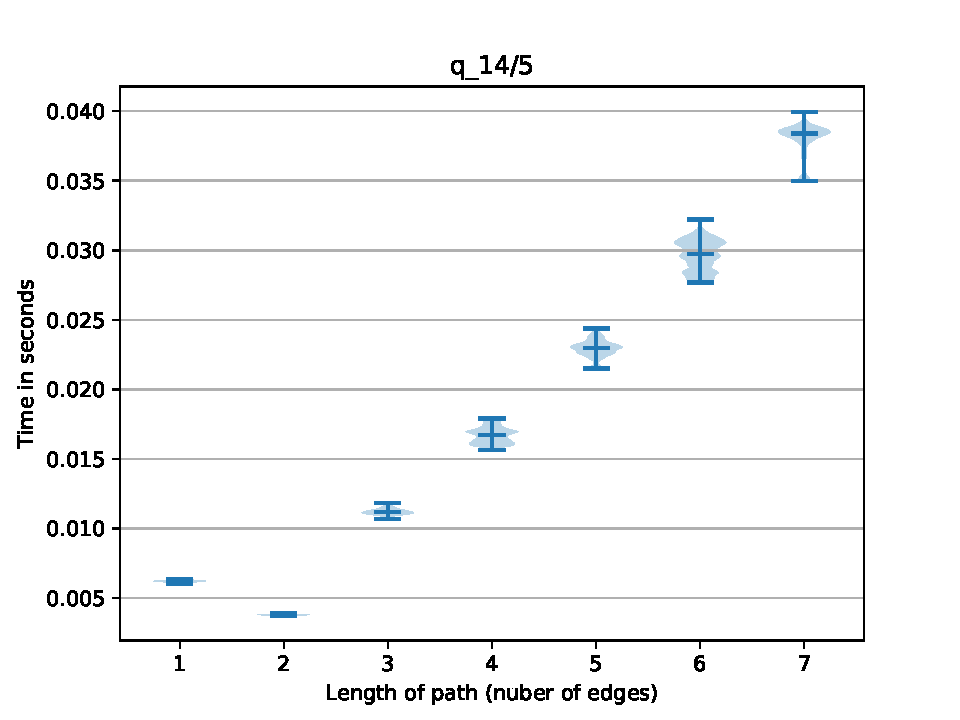
\includegraphics[width=0.48\textwidth]{data/res_graphics/q_14_5.pdf}
   \caption{Single path extraction}
\end{figure}

\subsubsection{Conclusion}

We can conclude that proposed algorithm is applicable for real-world data processing: the algorithm allows one both to solve reachability problem and to extract paths of interest in reasonable time even using na{\"i}ve implementation.  

\subsection{CFPQ Evaluation}

Comparison with matrix-based algorithm.

\subsubsection{Dataset}

Dataset for evaluation. 
It should be CFPQ\_Data\footnote{CFPQ\_Data is a dataset for CFPQ evaluation which contains both synthetic and real-world data and queries \url{https://github.com/JetBrains-Research/CFPQ\_Data}. Access date: 07.07.2020.}

\begin{table}
{
\rowcolors{2}{black!2}{black!10}
\begin{tabular}{|l|c|c|}
\hline
Graph & \#V & \#E \\
\hline
\hline 
eclass\_514en  & 120 926 & 484 646 \\
enzyme  & 358 434 & 144 9711 \\
geospecies  & 596 760 & 2 416 513 \\
go   & 1 188 340 & 4 820 728 \\
go-hierarchy & 1 780 956 & 7 228 358 \\
taxonomy & 2 308 385 & 9 369 511 \\
\hline
Aliases 1 & 6 442 630 & 24 465 430 \\
Aliases 2 & 4 834 262 & 12 366 973 \\
.... & 5 728 398 & 14 922 125 \\
\hline
\end{tabular}
}
\caption{Graphs for CFPQ evaluation}
\label{tbl:graphs_for_cfpq}
\end{table}



Same-generation queries, memory aliases.

\subsubsection{Results}

Results of evaluation.

Index creation.

{\setlength{\tabcolsep}{0.4em}
	\begin{table}
		\caption{RDFs query $G_1$ and $G_2$ (time is measured in seconds and memory is measured in megabytes)}
		\label{tbl:tableRDFQ1_appendix}
		\rowcolors{4}{black!2}{black!10}
		\small
		\begin{tabular}{| l | c | c | c | c |}
			\hline
			
			\multirow{2}{*}{Name}  & \multicolumn{2}{c|}{$G_1$} & \multicolumn{2}{c|}{$G_2$} \\
			\cline{2-5}
			                       & Tensors & RG\_CPU\textsubscript{path} & Tensors & RG\_CPU\textsubscript{path}	 \\
			\hline
			\hline
			eclass\_514en   & 0.254   & 0.195   & 0.227 & ...\\
			enzyme          & 0.035   & 0.029   & 0.036 & ...\\
			geospecies      & 0.091   & ...     & 0.001 & ...\\
			go-hierarchy    & 0.186   & 0.976   & 0.293 & ...\\
			go              & 1.676   & 1.286   & 1.368 & ...\\
			pathways        & 0.015   & 0.021   & 0.009 & ...\\
			taxonomy        & 5.366   & .....   & 3.282 & ...\\
			\hline
		\end{tabular}
	\end{table}
}


Paths extraction.

\subsubsection{Conclusion}

\section{Conclusion and future work}
In this paper, we shown how the context-free path query evaluation w.r.t. the relational and the single-path query semantics can be reduced to the calculation of matrix transitive closure. Also, we provided a formal proof of the correctness of the proposed reduction. In addition, we introduced an algorithm for computing this transitive closure, which allows us to efficiently apply GPGPU computing techniques. Finally, we shown the practical applicability of the proposed algorithm by running different implementations of our algorithm on real-world data.

We can identify several open problems for further research. In this paper we have considered only two semantics of context-free path querying but there are other important semantics, such as all-path query semantics~\cite{hellingsPathQuerying} which requires to present all paths for all triples $(A,m,n)$. Context-free path querying implemented with algorithm~\cite{GLL} can answer the queries in all-path query semantics by constructing a parse forest. It is possible to construct a parse forest for a linear input by matrix multiplication~\cite{okhotin_cyk}. Whether it is possible to generalize this approach for a graph input is an open question.

In our algorithm, we calculate the matrix transitive closure naively, but there are algorithms for the transitive closure calculation, which are asymptotically more efficient. Therefore, the question is whether it is possible to apply these algorithms for the matrix transitive closure calculation to the problem of context-free path querying.

Also, there are Boolean grammars~\cite{okhotinBoolean}, which have more expressive power than context-free grammars. Boolean path querying is an undecidable problem~\cite{hellingsRelational} but our algorithm can be trivially generalized to work on boolean grammars because parsing with boolean grammars can be expressed by matrix multiplication~\cite{okhotin_cyk}. It is not clear what a result of our algorithm applied to Boolean grammars would look like. Our hypothesis is that it would produce the upper approximation of a solution.

From a practical point of view, matrix multiplication in the main loop of the proposed algorithm may be performed on different GPGPU independently. It can help to utilize the power of multi-GPU systems and increase the performance of context-free path querying.

There is an algorithm~\cite{apspGPU} for transitive closure calculation on directed graphs which generalized to handle graph sizes inherently larger then the DRAM memory available on the GPU. Therefore, the question is whether it is possible to apply this approach to the matrix transitive closure calculation in the problem of context-free path querying.

\setmonofont[Mapping=tex-text]{CMU Typewriter Text}
\bibliographystyle{ugost2008ls}
\bibliography{diploma.bib}
\end{document}